\documentclass{iopart}
\usepackage{iopams}
\usepackage{braket,amsmath,color,graphicx,cite}
\usepackage[margin=2cm]{geometry}
\usepackage[colorlinks,linkcolor={blue},citecolor={blue}]{hyperref}
\bibliographystyle{unsrt}
\allowdisplaybreaks
\begin{document}

\title{Kondo frustration via charge fluctuations: a route to Mott localisation}

\author{Abhirup Mukherjee$^{1}$, N. S. Vidhyadhiraja$^{2}$, A. Taraphder$^{3}$ and Siddhartha Lal$^{1*}$}
\eads{\mailto{am18ip014@iiserkol.ac.in}, \mailto{raja@jncasr.ac.in}, \mailto{arghya@phy.iitkgp.ernet.in}, \mailto{slal@iiserkol.ac.in}}

\address{$^1$Department of Physical Sciences, Indian Institute of Science Education and Research-Kolkata, W.B. 741246, India}

\address{$^*$Corresponding author.}

\address{$^2$Theoretical Sciences Unit, Jawaharlal Nehru Center for Advanced Scientific Research, Jakkur, Bengaluru 560064, India}

\address{$^3$Department of Physics, Indian Institute of Technology Kharagpur, Kharagpur 721302, India}

\date{\today}

\begin{abstract}
We propose a minimal effective impurity model that captures the phenomenology of the Mott-Hubbard metal-insulator transition (MIT) of the half-filled Hubbard model on the Bethe lattice in infinite dimensions as observed by dynamical mean field theory (DMFT). This involves extending the standard Anderson impurity model Hamiltonian to include an explicit Kondo coupling $J$, as well as a local on-site correlation \(U_b\) on the conduction bath site connected directly to the impurity. For the case of attractive local bath correlations ($U_{b}<0$), the extended Anderson impurity model (e-SIAM) sheds new light on several aspects of the DMFT phase diagram. For example, the $T=0$ metal-to-insulator quantum phase transition (QPT) is preceded by an excited state quantum phase transition (ESQPT) where the local moment eigenstates are emergent in the low-lying spectrum. Long-ranged fluctuations are observed near both the QPT and ESQPT, suggesting that they are the origin of the quantum critical scaling observed recently at high temperatures in DMFT simulations. The \(T=0\) gapless excitations at the QCP display particle-hole interconversion processes, and exhibit power-law behaviour in self-energies and two-particle correlations. These are signatures of non-Fermi liquid behaviour that emerge from the partial breakdown of the Kondo screening.
\end{abstract}

\maketitle


\section{Introduction}

The rich physics of metal-insulator transitions in strongly correlated systems has been an active subject of study for quite some time~\cite{Mott_RMP_1968,milligan_1985,imada1998metal}, yet much still remains to be understood. It involves diverse aspects such as spin and charge fluctuations, quasiparticle renormalisation effects, anomalous metallic phases and unconventional superconductivity, and has been studied using an equally diverse array of methods like mean-field theory, renormalisation group approaches, numerical techniques like exact diagonalisation, quantum Monte Carlo and dynamical mean-field theory, and many others. In particular, dynamical mean-field theory (DMFT)~\cite{kuramoto1987,Cox1988,metzner_volhardt_1989,zhang_1993,georges1996,parcollet_2004,maier_2005,kotliar_2006,ohashi_2008} obtains an exact solution of the Mott metal-insulator transition (MIT) for the 1/2-filled Hubbard model~\cite{Mott_1949,gutzwiller_1963,kanamori_1963,hubbard1963electron,brinkman_rice_1970} on the Bethe lattice with infinite coordination number, in terms of an Anderson impurity model with a self-consistently determined bath obtained by requiring, in an iterative manner, that its local Greens function be equal to that of the impurity site. The above-mentioned transition can be captured by the local spectral function through (i) the continuous appearance of a Mott gap, followed by (ii) the sharpening and vanishing of the central Kondo resonance. These two features are often referred to, respectively, as the Mott-Hubbard~\cite{hubbard1963electron} and Brinkman-Rice~\cite{brinkman_rice_1970} scenarios of the Mott MIT. The exact nature of the solution arises from the fact that all non-local contributions to the lattice self-energy are observed to vanish upon taking the limit of an infinite coordination number for the lattice model. 
Thus, the simplification is that the dynamics of any local site on the lattice is determined completely by a quantum impurity problem~\cite{georges1996,Logan_2015}.
It must also be noted that this exact solution precludes any long-range order in the system, and corresponds to the case of a maximally frustrated Hubbard model involving long-range and frustrating inter-site hopping such that both the metallic and insulating phases remain paramagnetic~\cite{vucicevic_2013}.
Due to the exact and non-perturbative nature of the DMFT solution for the MIT in \(d=\infty\), the method has been extended to models of strongly correlated electrons in finite spatial dimensions~\cite{park2008,rohringer_2018,maier_2005}, as well as the study of the electronic properties of various correlated materials ~\cite{lichenstein_1998,kotliar_2006,held_2007_ldadmft}.

Despite this progress, a key aspect of the DMFT solution for the Hubbard model in $d=\infty$ remains to be understood. During the search for a self-consistent impurity model, the conduction bath is modified drastically in order to become correlated~\cite{held2008}. The numerical implementation of self-consistency, however, precludes a deeper understanding of the precise nature of the correlations present in the conduction bath of the impurity model, and its implications for the electron dynamics of the associated bulk lattice (Hubbard) model. Indeed, as we demonstrate below, our work paves the way for a more insightful exploration of the physics of the Mott Hubbard transition in strongly correlated electronic systems. Further, it has considerable consequences for the development of functional quantum materials and next-generation quantum technologies. Below, we lay out the specific questions addressed by us, and summarise our results at the end of this section.
\begin{itemize}
	\item[i.] Is there a minimal but effective quantum impurity model Hamiltonian that describes the Mott MIT of the $1/2$-filled Hubbard model on the Bethe lattice in \(d=\infty\)? Finding such an impurity model would also reduce the considerable computational effort that is presently required in self-consistent approaches.
	\item[ii.] What are the fluctuations that destroy the metal and lead to the insulating phase? Can we obtain a universal theory for these competing tendencies?
	\item[iii.] The coexistence of metallic and insulating phases at $T=0$ within DMFT shows that the insulating solution is present within the many-body spectrum of the metallic phase. Can an associated impurity model Hamiltonian display the emergence of the insulating state prior to the transition? Analytic insight of this kind is particularly important because approaching a coexistence region numerically is often fairly tricky.
	\item[iv.] Is it possible to obtain a low-energy theory for the local gapless excitations precisely at the MIT, where the metal is on the brink of destruction? How do these excitations compare with those of the local Fermi liquid, e.g., in terms of self-energies and two-particle correlation functions?
\end{itemize}
Obtaining answers to these questions would go a long way towards understanding the dominant fluctuations at the heart of the Mott transition and the physical processes that become important as one approaches it. It would also help in understanding the mechanism of DMFT's search for the self-consistent impurity model within the space of Anderson impurity models.

The essence of our approach is to model phenomenologically the lattice self-energy obtained from DMFT in the form of additional bath correlations within an extended Anderson impurity model.
In addition to the usual on-site repulsion ($U$) and single-particle hybridisation ($V$) between the impurity and the conduction bath of the Anderson impurity model (eq.~\eqref{basic-siam}), we introduce (i) an additional on-site correlation ($U_{b}$) on the bath site with which the impurity couples, and (ii) an antiferromagnetic Kondo coupling ($J$) between the impurity and the conduction bath (eq.~\eqref{GIAM-ham}). 
We note that a similar impurity model-based approach was taken towards understanding the physics of the heavy fermions several years ago by Si and Kotliar~\cite{si_kotliar_1993,kotliarsi_1993}. 
We postpone a comparison of our work with theirs to the discussions section. The rest of the work is structured as follows. Sec.~\eqref{def-ham} describes the extended model that we will study, and the unitary renormalisation group (URG) method that we employ to study it is presented in Sec.~\eqref{section-urg}. In Sec.~\eqref{urg-theory} and \eqref{desc-mit}, we describe the phase diagram and various characteristics of the impurity phase transition. In Sec.~\eqref{dmft}, we use our extended model to explain various features of the coexistence region observed in DMFT. In Sec.~\eqref{excitations}, we describe the effect of the impurity on the low-lying excitations of the bath, near and at the transition. We conclude in Sec.~\eqref{concl} with some discussions and possible future directions. For the convenience of readers, we first present below a brief summary of our main results.

\subsection*{\bf Summary of our main results}

\begin{itemize}
\item {\it Presence of a local metal-insulator transition}: At a critical value of the parameter $r=-U_{b}/J$, the effective impurity model shows a transition from a Kondo screened phase into an unscreened local moment phase. The quantum critical point (QCP) involves a degeneration of the Kondo singlet and the local moment states.
\item {\it The physics of Kondo screening and local pairing drives the transition:}
The transition involves the frustration of the Kondo screening of the impurity by enhanced local pairing fluctuations in the bath and can be described by a universal theory written in terms of $J$ and $U_b$.
\item {\it Emergence of insulating solutions in the metallic phase:}
Our analysis reveals that at a certain value of the parameter $r$ prior to the transition, the single-particle hybridisation parameter ($V$) turns irrelevant (in the RG sense), and this leads to the emergence of the local moment solutions within the many-particle spectrum through an excited state quantum phase transition (ESQPT).
\item {\it Critical fluctuations and the coexistence region}: 
We observe the appearance of long-ranged quantum fluctuations extending into the conduction bath in the vicinity of both the ESQPT at $r=r_{c1}$ and QPT at $r=r_{c2}$. We believe that these are the likely origin of the critical fluctuations observed above the finite temperature second-order critical point in DMFT~\cite{terletska_mott_2011,vucicevic_2013}. The two-step process at $T=0$ also provides a natural explanation for the coexistence of metallic and insulating features in the phase diagram, in the regime $r_{c1}<r<r_{c2}$.
\item {\it Emergence of non-Fermi liquid excitations at the QCP}:
Precisely at the QCP, the local  Fermi liquid is replaced by a quasi-local non-Fermi liquid (NFL) that spans the impurity, zeroth and first sites of the conduction bath. The NFL results from a degeneracy between the local moment and singlet states and leads to (i) ``Andreev scattering" of incoming states into orthogonal outgoing states, (ii) anomalous power-law behaviour in the self-energies and two-particle correlations with universal exponents, and (iii) a fractional entanglement entropy of the impurity.
\item {\it Correlated Fermi liquid excitations in the Hubbard sidebands}:
A many-body perturbation theoretic treatment of the Hubbard sidebands reveals that they are comprised of the holon-doublon excitations created by the hybridisation of the impurity site with the conduction bath. These excitations consist of decoupled local Fermi liquids for the holons and doublons at the lowest order, which, at higher orders, become coupled via correlated holon-doublon scattering between impurity and bath.
\end{itemize}

\section{Model Hamiltonian and method}

\subsection{The extended Anderson impurity model}
\label{def-ham}

The single-impurity Anderson model (SIAM)~\cite{anderson_1961,anderson_1978} consists of a single impurity site with local repulsive correlation \(U\) hybridising with a non-interacting fermionic conduction bath through a (momentum-independent) single-particle transfer whose coupling is \(V\). For the case of a half-filled impurity site, the Hamiltonian of the SIAM is given by
\begin{eqnarray} 
	\mathcal{H}_\text{A} = -\frac{U}{2} \left(\hat n_{d \uparrow} - \hat n_{d \downarrow}\right)^2 + \sum_{\vec k,\sigma} \epsilon_{\vec k} \tau_{\vec k,\sigma} + V\sum_\sigma \left(c^\dagger_{d\sigma}c_{0\sigma} + \text{h.c.}\right),
	\label{basic-siam}
\end{eqnarray}
where \(\tau_{\vec k,\sigma} \equiv c^\dagger_{\vec k,\sigma}c_{\vec k,\sigma} - 1/2\) indicate the occupancy of the single-particle momentum state \(\ket{\vec k}\). Also, \(c_{d\sigma}\) and \(c_{0\sigma} = \sum_k c_{k\sigma}\) are the fermionic annihilation operators of spin \(\sigma\) for the impurity and conduction bath site to which it couples (henceforth referred to as the {\it zeroth site}) respectively.  The conduction bath is typically considered to possess a constant (i.e., energy-independent) density of states. 

The SIAM (along with its \(U \to \infty\) limit, the Kondo model) has been studied using several analytical and numerical techniques~\cite{anderson1969exact,anderson1970exact,anderson1970,haldane1978scaling,jefferson_1977,wilson1975,hrk_wilson_1980,andrei_1980,andreiKondoreview,Wiegmann_1981,tsvelickKondoreview,kotliar_1996,Duki_2011,borda_2008,streib_2013,anirban_kondo}. 
The general conclusion for the positive \(U\) case at \(T=0\) is that on the particle-hole symmetric (that is, half-filled) line, the impurity local moment is always screened by the conduction electrons (referred to as the Kondo cloud~\cite{sorensen_erik_affleck_1996,affleck_ian_2001,simon_pascal_2003,martin2010,martin2019,Goldhaber-Gordon1998,Cronenwett1998,Schmid_Weis1998,pustilnik_glazman_2004,Borzenets2020,neel_berndt_2008,Zhao2005}). Enhanced spin-flip scattering at low-energies leads to the formation of a macroscopic singlet ground state and local Fermi liquid gapless excitations~\cite{nozaki2012,mora_2015}.
In order to enhance the SIAM, we introduce two extra two-particle interaction terms into the Hamiltonian:
\begin{itemize}
	\item a spin-exchange term \(J \vec{S}_d\cdot\vec{S}_0\) between the impurity spin \(\vec S_d\) and the spin \(\vec S_0\) of the zeroth site, and 
	\item a local particle-hole symmetric correlation term \(-U_b \left(\hat n_{0 \uparrow} - \hat n_{0 \downarrow}\right)^2\) on the bath zeroth site.
\end{itemize}

With these additional terms, the Hamiltonian of the {\it extended single-impurity Anderson model} (henceforth referred to as the e-SIAM) is, at particle-hole symmetry, given by
\begin{eqnarray}
	\label{GIAM-ham}
	\mathcal{H}_\text{E-A} = \mathcal{H}_\text{A} + J \vec{S}_d\cdot\vec{S}_0 - \frac{1}{2}U_b \left(\hat n_{0 \uparrow} - \hat n_{0 \downarrow}\right)^2~.
\end{eqnarray}
All the terms in the Hamiltonian have been depicted schematically in the left panel of Fig.~\eqref{zeromode-bare}. The additional interaction terms \(J\) and \(U_b\) enjoy particle-hole, SU(2)-spin and U(1)-charge symmetries. The e-SIAM Hamiltonian (eq.~\eqref{GIAM-ham}) therefore preserves all the local symmetries of the half-filled Hubbard model on a lattice, and can potentially serve as an effective auxiliary quantum impurity model (with a correlated bath) describing the local physics of the latter.

\subsection{The unitary renormalisation group method}\label{section-urg}
In order to obtain the various low-energy phases of the e-SIAM, we perform a scaling analysis of the associated Hamiltonian (eq.~\eqref{GIAM-ham}) using the recently developed unitary renormalisation group (URG) method \cite{anirbanurg1,anirbanurg2}. The method has been applied successfully on a wide variety of problems of correlated fermions~\cite{santanukagome,1dhubjhep,anirbanmott2,anirbanmott1,siddharthacpi,anirban_kondo,Patra_2023,anirbanurg1,anirbanurg2}. The method proceeds by resolving quantum fluctuations in high-energy degrees of freedom, leading to a low-energy Hamiltonian with renormalised couplings and new emergent degrees of freedom. Typically, for a system with Fermi energy \(\epsilon_F\) and bandwidth \(D_0\), the sequence of isoenergetic shells \(\left\{D_{(j)}\right\}, D_{(j)}\in \left[\epsilon_F, D_0\right] \) define the states whose quantum fluctuations we sequentially resolve. The momentum states lying on shells \(D_{(j)}\) that are far away from the Fermi surface comprise the UV states, while those on shells near the Fermi surface comprise the IR states. This scheme is shown in the right panel of Fig.~\eqref{zeromode-bare}.

\begin{figure}[!htb]
	$\vcenter{\hbox{\includegraphics[width=0.45\textwidth]{esiam_bare.pdf}}}$
	\hspace*{\fill}
	$\vcenter{\hbox{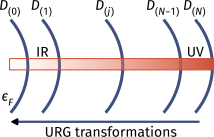
\includegraphics[width=0.3\textwidth]{urg-scheme.pdf}}}$
	\caption{{\it Left:} Schematic 1D representation of the extended SIAM Hamiltonian. The red sphere is the impurity site with on-site Hubbard term \(U\). It is connected via two couplings \(V\) and \(J\) to the bath zeroth site (large blue sphere) that has its own on-site Hubbard term \(U_b\). The small blue spheres make up the rest of the bath, connected through the single-particle hopping \(t\). {\it Right:} High energy - low energy scheme defined and used in the URG method. The states away from the Fermi surface form the UV subspace and are decoupled first, leading to a Hamiltonian which is more block-diagonal and comprised of only the IR states near the Fermi surface.}
	\label{zeromode-bare}
\end{figure}

As a result of the URG transformations, the Hamiltonian \(H_{(j)}\) at a given RG step \(j\) involves scattering processes between the \(k-\)states that have energies lower than \(D_{(j+1)}\). The unitary transformation \(U_{(j)}\) is then defined so as to remove the number fluctuations of the currently most energetic set of states \(D_{(j)}\)~\cite{anirbanurg1,anirbanurg2}:
\begin{eqnarray}
	H_{(j-1)} = U_{(j)} H_{(j)} U^\dagger_{(j)}~, \text{such that} ~\left[H_{(j-1)}, \hat n_{j}\right] =0~.
\end{eqnarray}
The eigenvalue of $\hat{n}_{j}$ has, thus, been rendered an integral of motion (IOM) under the RG transformation.

The unitary transformations can be expressed in terms of a generator \(\eta_{(j)}\) that has fermionic algebra~\cite{anirbanurg1,anirbanurg2}:
\begin{eqnarray}
	\label{unitary}
	U_{(j)} = \frac{1}{\sqrt 2}\left(1 + \eta_{(j)} - \eta_{(j)}^\dagger\right)~,~ \quad\left\{ \eta_{(j)},\eta_{(j)}^\dagger \right\} = 1~,
\end{eqnarray}
where \(\left\{\cdot\right\}\) is the anticommutator. The unitary operator \(U_{(j)}\) that appears in Eq.~\eqref{unitary} can be cast into the well-known general form \(U = e^\mathcal{S}, \mathcal{S} = \frac{\pi}{4}\left( \eta^\dagger_{(j)} - \eta_{(j)} \right)\) that a unitary operator can take, defined by an anti-Hermitian operator \(\mathcal{S}\). The generator \(\eta_{(j)}\) is given by the expression~\cite{anirbanurg1,anirbanurg2}
\begin{eqnarray}
	\eta^\dagger_{(j)} = \frac{1}{\hat \omega_{(j)} - \text{Tr}\left(H_{(j)} \hat n_{j}\right) } c^\dagger_{j} \text{Tr}\left(H_{(j)}c_{j}\right)~.
\end{eqnarray}
The operators \(\eta_{(j)},\eta^\dagger_{(j)}\) behave as the many-particle analogues of the single-particle field operators \(c_j,c^\dagger_j\) - they change the occupation number of the single-particle Fock space \(\ket{n_j}\).  The important operator \(\hat \omega_{(j)}\) originates from the quantum fluctuations that exist in the problem because of the non-commutation of the kinetic energy terms and the interaction terms in the Hamiltonian:
\begin{eqnarray}
	\hat \omega_{(j)} = H_{(j-1)} - H^i_{(j)}~.
	\label{omega}
\end{eqnarray}
\(H^i_{(j)}\) is the part of \(H_{(j)}\) that commutes with \(\hat n_j\) but does {\it not} commute with at least one \(\hat n_l\) for \(l < j\). The RG flow continues up to energy \(D^*\), where a fixed point is reached from the vanishing of the RG function. 
Detailed comparisons of the URG with other methods (e.g., the functional RG, spectrum bifurcation RG etc.) can be found in Refs.~\cite{anirbanmott1,anirbanurg1}. More information on the unitary RG method is provided in Section 1 of the Supplementary Materials~\cite{supp_mat}.

\section{\(T=0\) scaling theory for the e-SIAM}
\label{urg-theory}

\subsection{URG equations for the e-SIAM}

The derivation of the RG equations for the extended Anderson impurity model (e-SIAM) Hamiltonian is shown in Section 2 of the Supplementary Materials~\cite{supp_mat}. The bath coupling \(U_b\) is marginal. We provide below the RG equations of the remaining couplings for a given quantum fluctuation scale \(\omega\):
\begin{align}
	\Delta U &= 4V^2 n_j\left(\frac{1}{d_1} - \frac{1}{d_0}\right) - n_j\frac{J^2}{d_2},\nonumber\\
	\Delta V &= -\frac{3n_j V}{8}\left[J\left(\frac{1}{d_2} + \frac{1}{d_1}\right) +  \frac{4U_b}{3}\sum_{i=1}^4 \frac{1}{d_i}\right],\label{rg-eqn}\\
	\Delta J &= -\frac{n_j J\left(J + 4U_b\right)}{d_2}~,\nonumber
\end{align}
where the denominators \(d_i\) are given by
\begin{eqnarray}\label{rg-eqtn1}
	d_0 = \omega - \frac{D}{2} + \frac{U_b}{2} - \frac{U}{2},~d_1 = \omega - \frac{D}{2} + \frac{U_b}{2} + \frac{U}{2} + \frac{J}{4}~,\\
	d_2 = \omega - \frac{D}{2} + \frac{U_b}{2} + \frac{J}{4}~,d_3 = \omega - \frac{D}{2} + \frac{U_b}{2}~.
\end{eqnarray}
The symbols used in the RG equations have the following meanings: \(\Delta U\) represents the renormalisation of the coupling \(U\) in going from the \(j^\text{th}\) Hamiltonian to the \(\left( j-1 \right) ^\text{th}\) Hamiltonian by decoupling the isoenergetic shell at energy \(D_{(j)}\) (see right panel of Fig.\eqref{zeromode-bare}). \(n_j\) is the number of electronic states on the shell \(D_{(j)}\). We note that the labels \(U_0,J_0,V_0\) that appear in various figures (and elsewhere in the text) represent the bare values of the associated couplings \(U,J\) and \(V\). The RG equations reduce, in the perturbative regime of the couplings $U, V$ and $J$, to the well-known ``poor man's" scaling forms obtained for the  SIAM~\cite{haldane1978scaling} and the single-channel Kondo model~\cite{anderson1970} respectively.

 The RG fixed point Hamiltonian describes the low-energy phase of the system. In general, if the RG fixed point is reached at an energy scale \(D^*\), the fixed point Hamiltonian \(\mathcal{H}^*\) is obtained simply from the fixed point values of the couplings (and by noting that the states above \(D^*\) are now part of the IOMs):
\begin{eqnarray}
	\label{fixed-point-ham}
	\mathcal{H}^* = \sum_{\sigma,\vec k}^{|\epsilon_{\vec k}| < D^*} \epsilon_{\vec k} \tau_{\vec k,\sigma} + V^*\sum_\sigma \left( c^\dagger_{d\sigma}c_{0\sigma} + \text{h.c.}\right) + J^* \vec{S}_d\cdot\vec{S}_0\nonumber - \frac{1}{2}U^*\left(\hat n_{d \uparrow} - \hat n_{d \downarrow}\right)^2 - \frac{1}{2}U_b \left(\hat n_{0 \uparrow} - \hat n_{0 \downarrow}\right)^2~.
\end{eqnarray}
The fixed point values of the couplings are obtained by solving the RG equations numerically.

\begin{figure}[!htbp]
	$\vcenter{\hbox{\includegraphics[width=0.48\textwidth]{phase-map-MIT.pdf}}}$
	\hspace*{\fill}
	$\vcenter{\hbox{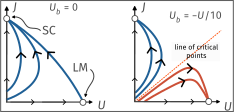
\includegraphics[width=0.48\textwidth]{rg-flows-schematic.pdf}}}$
	\caption{{\it Left:} Phase diagram of the e-SIAM, in the space of \(r\) and \(J_0/D_0\). \(U_b\) is set to \(-U_0/10\). The various phases are described in the text. {\it Right:} Schematic nature of RG flows for \(U_b=0\) and \(U_b = -U/10\). Blue curves represent RG flows towards the strong-coupling (SC) fixed point, while red curves represent RG flows towards the local moment (LM) fixed point.}
	\label{phase-diag}
\end{figure}

\subsection{Phase diagram}

We will work in the low-energy regime where the quantum fluctuation scale \(\omega\) is such that all the denominators are negative: \(d_i < 0 ~\forall~i\). Moreover, we constrain the impurity and local bath correlations (\(U\) and \(U_b\) respectively) through the relation \(U_{b} = -U/10\). While the precise value of the factor of \(1/10\) is unimportant, we have 
chosen a factor considerably smaller than 1 in order to demonstrate that an interesting body of results can be obtained with a value of $|U_{b}|$ that is much smaller than that of $U$. Further, the negative sign in the above relation is significant, as we shall see below that the MIT is obtained for the case of \(U_b\) being negative (i.e., attractive on-site correlations on the zeroth site of the bath). The relation between $U_{b}$ and $U$ is motivated on phenomenological grounds such that the MIT occurring in the bulk lattice model (obtained upon increasing the on-site Hubbard repulsion to large values) corresponds, in the auxiliary model mapping within DMFT, to the local MIT observed upon tuning the impurity correlation $U$ (and the related bath correlation \(U_b\)) within the proposed effective impurity model Hamiltonian. The physical significance of attractive on-site correlations in the bath lies in providing a mechanism for the frustration of Kondo screening (in the RG equation for an antiferromagnetic Kondo coupling $J(>0)$, eq.~\eqref{rg-eqn}) within an Anderson impurity coupled to a single channel of conduction electrons. We provide a detailed discussion of this point in the concluding section of our work.

\begin{table*}[!htbp]
\centering
\begin{tabular}{|cl|c|c|}
\hline
& Regime & Low-energy effective Hamiltonian & impurity ground-state\\[5pt]
\hline
1. & \(0 < r < r_{c1}\) &  \(\text{K.E}^* + V^*\sum_\sigma \left( c^\dagger_{d\sigma}c_{0\sigma} + \text{h.c.}\right) + J^* \vec{S}_d\cdot\vec{S}_0\) & \(\frac{1}{\sqrt 2}\left(\ket{\uparrow_d}\ket{\downarrow_0} - \ket{\downarrow_d} \ket{\uparrow_0} + \ket{2_d}\ket{0_0} + \ket{0_d} \ket{2_0}\right)\)\\[10pt]
2. & \(r_{c1} < r < r_{c2}\) &  \(\text{K.E}^* + J^* \vec{S}_d\cdot\vec{S}_0 - \frac{1}{2}U_b \left(\hat n_{0 \uparrow} - \hat n_{0 \downarrow}\right)^2\) & \(\frac{1}{\sqrt 2}\left(\ket{\uparrow_d}\ket{\downarrow_0} - \ket{\downarrow_d} \ket{\uparrow_0}\right)\)\\[10pt]
3. & \(r_{c2} < r\) &  \(\text{K.E}^* - \frac{U^*}{2}\left(\hat n_{d \uparrow} - \hat n_{d \downarrow}\right)^2 - \frac{U_b}{2} \left(\hat n_{0 \uparrow} - \hat n_{0 \downarrow}\right)^2\) & \(\left\{ \ket{\uparrow_d},\ket{\downarrow_d}\right\}\)\\[5pt]
\hline
\end{tabular}
\caption{Effective Hamiltonians and ground-states of the three important parts of the phase diagram in Fig.~\eqref{phase-diag}. The ground-state is simplified to capture only the configuration of the impurity site and at most the bath zeroth site. \(\text{K.E.}^*\) represents the kinetic energy of the conduction electron states residing within the fixed point window \(D^*\).}
\label{phases-table}
\end{table*}

The phase diagram is shown in the left panel of Fig.~\eqref{phase-diag} in terms of the parameter $r=|U_{b}|/J$ (y-axis) and the ratio of the bare Kondo coupling ($J_{0}$) to the bare conduction bath bandwidth ($D_{0}$) (x-axis), we first define two important points in the space of couplings. These are values of the parameter \(r\) where there is a qualitative change in the nature of RG flows, and hence in the low-energy physics of the model
\begin{itemize}
	\item \(r = r_{c1} \left(= -\left(\frac{U_b}{J}\right)_{c1} = \frac{3}{20} = \left(\frac{U}{10 J}\right)_{c1}>0\right)\): At this point, the coupling \(V\) becomes irrelevant,
	\item \(r = r_{c2} \left(= -\left(\frac{U_b}{J}\right)_{c2} = \frac{1}{4} = \left(\frac{U}{10 J}\right)_{c2}\right)\): At this point, the coupling \(J\) also turns irrelevant. Note that $r_{c2} > r_{c1}$.
\end{itemize}
We will use these two values of the parameter $r$ as checkpoints around which we can describe the low-energy physics. 
There are three important parts in Fig.~\eqref{phase-diag}:
\begin{itemize}
	\item red region, \(0 < r < r_{c1}\): the \(J-V\) model; {\it \(V\) and \(J\) are both relevant, but $U$ is irrelevant}; spin and charge delocalisation on the impurity; spin-charge mixing in ground-state
	\item blue region, \(r_{c1} < r < r_{c2}\): the \(J-U_b\) model; {\it $J$ is relevant, but \(V\) and $U$ are both irrelevant}; charge localisation and spin delocalisation on the impurity; singlet ground-state
	\item violet region, \(r_{c2} < r\): the \(U-U_b\) model; {\it $U$ is relevant, but \(V\) and \(J\) are both irrelevant}; spin and charge localisation on the impurity; local moment ground-state. This phase describes a local Mott insulator on the impurity site, characterised by vanishing local double occupancy in ground state (black curve in left panel of Fig.~\ref{spec_func}).
\end{itemize}
Typical RG flows that lead to these phases are shown in Fig.~\eqref{rg-flow}. We also note that the grey region shown in the top right corner of Fig.\eqref{phase-diag} corresponds to a model in which all three couplings ($J$, $U$ and $V$) are RG irrelevant. We find, however, that this phase is an artefact of solving the RG equations for an impurity coupled to a finite-sized conduction bath, and it gradually disappears upon increasing the bath size.

\begin{figure*}[!htbp]
\centering
\includegraphics[width=\textwidth]{rg-flows-all.pdf}
\caption{Variation of couplings \(U,V\) and \(J\) along the RG transformations, for three values of the transition-tuning ratio \(r = -U_b/J_0\). The x-axis represents the distance of the running cutoff from the Fermi surface; the rightmost point is the first RG step (UV) and the leftmost point is the final RG step (IR). The red curves represent the flows for \(r < r_{c1}\), where both \(V\) and \(J\) are relevant. The blue curves represent the RG flows for \(r_{c1} < r < r_{c2}\), where \(J\) is relevant but \(V\) is irrelevant. The violet curves represent RG flows for \(r > r_{c2}\), where both \(V\) and \(J\) are irrelevant but \(U\) flows to a finite value.}
\label{rg-flow}
\end{figure*}

\subsection{Phase transition at \(r_{c2}\)}
The effective Hamiltonians and corresponding impurity ground-states for various phases have been listed in table ~\eqref{phases-table}. The variation in the ground state has been checked by numerically solving the fixed point Hamiltonian for various bare values of the couplings and is shown in the left panel of Fig.~\eqref{spec_func}.
A sharp change in the ground state from spin-singlet to local moment shows that the blue and violet phases are separated by an {\it impurity delocalisation-localisation transition} (black line in Fig.~\eqref{phase-diag}). The transition occurs at finite values of the correlations: \(r_{c2} = -\left(\frac{U_b}{J}\right)_{c2} = \frac{1}{4} = \left(\frac{U}{10 J}\right)_{c2}\). This is a stark contrast from the standard SIAM, where the transition can happen only at on-site correlation \(U \to\infty\). Therefore, the presence of the critical point at finite values of the various couplings transforms the landscape of RG phase diagram shown schematically in the right panel of Fig.~\eqref{phase-diag} (right panel): the RG flows split into two classes - those that flow towards the strong-coupling Kondo screened fixed point and those that flow towards the local moment fixed point.

By a simple rewriting of the RG equation for \(J\) (eq.~\eqref{rg-eqn}), the impurity transition can be seen to arise from a competition between the Kondo screening physics of \(J\) and the local pairing physics of \(U_b\):
\begin{eqnarray}
\Delta J = \overbrace{\frac{(J + 2U_b)^2 n_j}{|d_{2}|}}^\text{usual Kondo physics} - \overbrace{\frac{(2U_b)^2 n_j}{|d_{2}|}}^\text{competing pairing physics}~,
\end{eqnarray}
where $d_{2}=\omega - D/2 + U_b/2 + J/4$. The competition between the effective Kondo term \((J + 2U_b)^2\) and the competing pairing term \(-4U_b^2\) leads to the presence of two stable phases - one that is Kondo screened and one that remains unscreened.

In the DMFT treatment of the $1/2$-filled Hubbard model on the Bethe lattice in infinite dimensions, the vanishing of non-local contributions to the lattice self-energy means that the lattice Greens function can be computed self-consistently by solving a local quantum impurity problem~\cite{georges1996}. In the rest of the work, we provide extensive evidence that the local transition observed in the e-SIAM is very similar to the Mott MIT observed in DMFT. We conclude thereby that the e-SIAM models faithfully the round-trip excursions of an electron on the Bethe lattice, and that the impurity phase transition observed in the e-SIAM offers a local description of the Mott MIT in the bulk Hubbard model. With this evidence in mind, we will henceforth refer to the transition at \(r_{c2}\) as a {\it local metal-insulator transition}.


\subsection{The case of repulsive \(U_b\)}
Henceforth, we will only consider the case of attractive \(U_b\) (\(U_b > 0\)), because that is the regime in which an impurity phase transition is realised at finite values of the couplings. However, before moving on, we will comment briefly on the effects of a repulsive \(U_b\) (\(U_b > 0\)). From the RG equation for \(J\) in eq.~\ref{rg-eqn}, we see that \(\Delta J\) is always positive for \(U_b > 0\). Moreover, something similar happens in the RG equation for \(V\), where the two terms in the square brackets now enforce each other (\(J\) and \(U_b\) now have the same sign). Together, they indicate that there will not be any Kondo destruction in the case of \(U_b > 0\), and the only fixed points are the weak-coupling one (\(J^* = 0\)) and the strong coupling one (\(J^* = \infty\)); there is no local moment phase. This case is therefore adiabatically connected to the case of \(U_b = 0\).


\section{Descriptors of the local MIT}
\label{desc-mit}

The present section gives more clarity on the nature of the impurity phase transition in the form of additional descriptors of the transition such as impurity spectral function and measures of entanglement, computed from the e-SIAM Hamiltonian. Throughout the rest of the work, we have set the value of the coupling \(V\) equal to the Kondo coupling \(J\) while generating the quantitative plots.

\subsection{Evolution of the impurity spectral function}

The impurity spectral function of the standard SIAM (eq.~\eqref{basic-siam}) always displays a central peak at finite values of \(U\) (along with Hubbard sidebands at sufficiently large \(U\)), indicating the presence of gapless local Fermi liquid excitations on the impurity site~\cite{wilson1975,nozieres1974fermi,costi_hewson_1990}. To demonstrate the impurity localisation transition, we compute the impurity local spectral function of the e-SIAM (eq.~\eqref{GIAM-ham}). This involves numerically diagonalising the effective Hamiltonian at various energy scales along the RG flow and computing the spectral weight at a range of frequencies from UV to IR. We find that the spectral function (shown in the right panel of Fig.~\eqref{spec_func}) displays three notable features, in agreement with DMFT results~\cite{georges1996}:
\begin{itemize}
	\item The appearance of a {\it preformed gap} (flattening of spectral function between the central peak and sidebands) as \(r\) crosses \(r_{c1} \left(= -\left(\frac{U_b}{J}\right)_{c1} = \frac{3}{20} = \left(\frac{U}{10 J}\right)_{c1}\right)\): The preformed optical gap simply indicates the separation of the spin (central peak) and charge (sidebands) degrees of freedom beyond \(r_{c1}\). This separation is brought about by the irrelevance of \(V\). We note that the consequences of an irrelevant hybridisation \(V\) can be accounted for in many-body perturbation theory, leading to ``in-gap" processes within the optical gap of the impurity spectral function~\cite{nozieres_dmft}. However, we expect that such contributions will be small, and cannot fill in the optical gap observed in Fig.\ref{spec_func} completely.
	\item The sharpening of the central peak, and concomitant increase in the preformed gap, as $r$ is increased in the range $r_{c1} < r < r_{c2}$.
	\item The vanishing of the central peak and appearance of a {\it hard gap} as \(r\) crosses \(r_{c2}\): The irrelevance of \(J\) beyond \(r_{c2}\) destroys the Kondo screening and localises the impurity moment. This involves the destabilisation of the singlet ground state, and the stabilisation of the local moment states in its place.
\end{itemize}

\begin{figure}[!htb]
	\includegraphics[width=0.45\textwidth]{corrs_gs.pdf}
	\hspace*{\fill}
	\includegraphics[width=0.45\textwidth]{spectral-function.pdf}
	\caption{{\it Left:} Overlap of the RG fixed point ground state \(\ket{\Psi}_\text{gs}\) with the spin-singlet state \(\ket{\text{SS}}\), the zero charge member of the charge triplet states \(\ket{\text{CT}}\) and the local moment states \(\ket{\text{LM}}\), for all three regimes of the model. The black curve corresponds to the double occupancy on the impurity site and is observed to be strongly suppressed beyond $r_{c1}$. Beyond the critical point \(r_{c2} = 0.25\), the overlaps with the entangled states vanish, indicating the transition to a decoupled local moment. {\it Right:} Variation of the impurity spectral function from \(r = 0\) to \(r > r_{c2}\). At small \(r\), the central peak is broad, but at larger \(r\), it sharpens, and the difference in spectral weight is used in creating the Hubbard sidebands. For \(r > r_{c2}\), the central peak vanishes.}
	\label{spec_func}
\end{figure}

These features are also reflected in ground-state correlation measures like spin-flip and charge isospin-flip correlations (see left panel of Fig.~\eqref{gstate-correlations}), which are defined as follows:
\begin{eqnarray}
\hspace*{-1cm}
\frac{1}{2}\left(\braket{S_{i}^{+}S_{j}^{-}} + \text{h.c.}\right) = \frac{1}{2}\left(\braket{c^\dagger_{i \uparrow}c_{i \downarrow}c^\dagger_{j \downarrow}c_{j \uparrow}} + \text{h.c.}\right)~,~
\frac{1}{2}\left(\braket{C_{i}^{+}C_{j}^{-}} + \text{h.c.}\right) = \frac{1}{2}\left(\braket{c^\dagger_{i \uparrow}c^\dagger_{i \downarrow}c_{j \downarrow}c_{j \uparrow}} + \text{h.c.}\right)~.
\end{eqnarray}
At small values of \(r\), both the correlations are large as the ground-state has both spin and charge content (row 1 of table~\eqref{phases-table}). The subsequent decrease in the impurity-bath charge flip correlation (violet points of Fig.~\eqref{gstate-correlations}), and the simultaneous increase in the impurity-bath spin-flip correlation (red points of Fig.~\eqref{gstate-correlations}), can be attributed to the irrelevance of \(V\) at \(r\simeq r_{c1}\) and the appearance of the preformed gap in the spectral function. Beyond \(r_{c2}\), the spin-flip correlation sharply drops to zero due to the irrelevance of \(J\). They are replaced by intra-bath correlations like the charge isospin-flip correlation between the zeroth site and the first site (blue points of Fig.~\eqref{gstate-correlations}). Such intra-bath correlations are promoted by the bath on-site term \(U_b\). The sudden change in the nature of the ground state, and resulting correlations, at $r_{c2}$ indicates the presence of a quantum critical point whose nature will be analysed further in subsequent sections. 

\begin{figure}[!htb]
	\includegraphics[width=0.45\textwidth]{spin-charge-corr-full.pdf}
	\hspace*{\fill}
	\includegraphics[width=0.45\textwidth]{entanglement.pdf}
	\caption{{\it Left:} Variation of impurity-bath spin-flip correlation (red) and charge isospin-flip correlation (violet), as well as intra-bath charge isospin-flip correlation (blue), from \(r \sim 0\) to \(r > r_{c2}\). The imp.-bath isospin correlation vanishes at \(r_{c1}\), indicating the change in RG relevance of \(V\). The imp.-bath spin correlation vanishes at \(r_{c2}\), indicating the marginality of \(J\) at that point. The intra-bath correlation picks up after the transition, showing the decoupling of the impurity from the bath. {\it Right:} Variation of the geometric entanglement \(\varepsilon_\text{ss}\) (blue) w.r.t. the singlet state and that w.r.t the charge triplet zero state, \(\varepsilon_\text{ct}\) (red), with \(r\). The former becomes maximum (unity) at \(r_{c1}\), showing that the true ground state has no charge content. The latter discontinuously jumps to unity at \(r_{c2}\), therefore acting as an order parameter for the transition.}
	\label{gstate-correlations}
\end{figure}

\subsection{Using entanglement to track correlations across the transition}

We will now show that a certain measure of entanglement behaves as an order parameter for the transition. We can define a geometric measure of entanglement in terms of wavefunctions \(\ket{\psi_1}\) and \(\ket{\psi_2}\)~\cite{shimony1995degree,wei2003geometric,horodecki2009quantum}:
\begin{eqnarray}
	\varepsilon\left(\psi_1,\psi_2\right) = 1 - |\braket{\psi_1 | \psi_2}|^2~.
\end{eqnarray}
From this definition, if \(\ket{\psi_1}\) corresponds to a separable state, the entanglement content of the state \(\ket{\psi_2}\) is small if it's overlap with \(\ket{\psi_1}\) is large.
For brevity, we will use the notation \(\varepsilon_\text{ss} \equiv \varepsilon\left(\psi_\text{ss},\psi^{(2)}_\text{gs}\right), \varepsilon_\text{ct} \equiv \varepsilon\left(\psi_\text{ct},\psi^{(2)}_\text{gs}\right)\) to represent the geometric entanglement between the e-SIAM ground-state \(\ket{\psi_\text{gs}}\) and the singlet state \(\ket{\psi_\text{ss}}\) or the charge triplet zero state \(\ket{\psi_\text{ct}}\).
The latter two states are shown in Table \eqref{phases-table}.
The entanglement measures $\varepsilon_{\text{ss}}$ and $\varepsilon_{\text{ct}}$ can be related to the impurity Greens function through the following equation (details can be found in Sec. 3 of the Supplementary Materials~\cite{supp_mat}):
\begin{eqnarray}
	G_d(\omega) = \sum_n &\left[\left(1 - \varepsilon_\text{ss} \right) G_{\Phi_\text{ss},\Phi_\text{ss}}(\omega,n) + \left(1 - \varepsilon_\text{ct} \right) G_{\Phi_\text{ct},\Phi_\text{ct}}(\omega,n) \right.\nonumber \\
			     &\left.+ 2\sqrt{\left(1 - \varepsilon_\text{ss} \right)}\sqrt{\left(1 - \varepsilon_\text{ct} \right)} G_{\Phi_\text{ss},\Phi_\text{ct}}(\omega,n)\right]~,
	\label{greens-func}
\end{eqnarray}
where
\begin{eqnarray}
	G_{\psi_1,\psi_2}(\omega,n) = \frac{1}{2}\frac{\braket{\psi_1 | c_{d\sigma} | \Psi_n}\braket{\Psi_n | c^\dagger_{d\sigma} | \psi_2} + \text{h.c.}}{\omega + E_\text{gs} - E_n} + \frac{1}{2}\frac{\braket{\psi_1 | c^\dagger_{d\sigma} | \Psi_n}\braket{\Psi_n | c_{d\sigma} | \psi_2} + \text{h.c.}}{\omega - E_\text{gs} + E_n}~.
\end{eqnarray}

This expression displays that the evolution of the impurity Greens function $G_{d}$ 
with $r$ (and related correlation functions shown in the left panel of Fig.\eqref{gstate-correlations}) is dependent on that of the entanglement measures $\varepsilon_{\text{ss}}$ and $\varepsilon_{\text{ct}}$ (shown in the right panel of Fig.~\eqref{gstate-correlations}). 
Indeed, we find that the geometric entanglement \(\varepsilon_\text{ct}\) with the charge sector increases towards unity as the transition at \(r_{c2}\) is approached, and remains unity after the transition. A more sensitive measure is the singlet entanglement \(\varepsilon_\text{ss}\): it initially decreases to zero at \(r_{c1}\) owing to the irrelevance of \(V\), but rises discontinuously to unity at the transition and becomes equal to the charge entanglement in the local moment phase.
Therefore, \(\varepsilon_\text{ss}\) {\it acts as an order parameter} for the local MIT at \(r_{c2}\). We find that the cross-term \(\sqrt{\left(1 - \varepsilon_\text{ss} \right)}\sqrt{\left(1 - \varepsilon_\text{ct} \right)}\) decreases monotonically to zero with increasing \(r\) (not shown), displaying a continual decrease in the mixing of the spin and charge sectors and the {\it immobilisation of the doublons and holons on the impurity site}. 

In general, any one-particle or two-particle fluctuation \(\left<O_1 O_2^\dagger \right>\) that acts on the combined Hilbert space of the impurity and the zeroth site can be expressed in terms of these entanglement measures \(\varepsilon_\text{ss},\varepsilon_\text{ct}\). The detailed derivations and expressions are given in Section 3 of the Supplementary Materials~\cite{supp_mat}. As a demonstration, consider the spin-spin correlation $\langle S_{d}^{+}S_{0}^{-}\rangle$ between the impurity and the zeroth site shown in the left panel of Fig.~\eqref{gstate-correlations}. The general expression given in Section 3 of the Supplementary Materials~\cite{supp_mat} is of the form
\begin{eqnarray}
	\braket{S_{d}^{+}S_{0}^{-}} =& \left(1 - \varepsilon_\text{ss}\right) \braket{\Phi_\text{ss} | S_d^+ S_0^- | \Phi_\text{ss}} + \left(1 - \varepsilon_\text{ct}\right) \braket{\Phi_\text{ct} | S_d^+ S_0^- | \Phi_\text{ct}} \nonumber \\
				      &+ \sqrt{1 - \varepsilon_\text{ss}}\sqrt{1 - \varepsilon_\text{ct}}\left(\braket{\Phi_\text{ss} | S_d^+ S_0^- | \Phi_\text{ct}} + \braket{\Phi_\text{ct} | S_d^+ S_0^- | \Phi_\text{s}}\right)~.
\end{eqnarray}

From the expression given, we find that only the singlet overlap is non-zero, such that $\langle S_{d}^{+}S_{0}^{-}\rangle$ is directly proportional to the quantity \(1-\varepsilon_\text{ss}\). As the entanglement measure \(\varepsilon_\text{ss}\) increases towards the transition (right panel of Fig.~\eqref{gstate-correlations}), the quantity \(1 - \varepsilon_\text{ss}\) decreases, in turn leading to the decrease in the magnitude of the correlation observed in the left panel of Fig.~\eqref{gstate-correlations}. For another explicit connection between correlations and entanglement measures, we present relations between the quantum Fisher information (QFI)~\cite{Hauke2016} and many-particle Greens functions in Section 3 of the Supplementary Materials~\cite{supp_mat}. There, we also plot the QFI for a number of two-particle operators as a function of \(r\), notably the ones corresponding to the degree of compensation for the impurity (\(\braket{\vec{S}_d\cdot\vec{S}_0}\)) and the impurity magnetisation (\(\braket{S_d^z}\)).
These two quantities (and hence the corresponding QFI) are important because they track the local MIT and act as order parameters for the transition, and the QFI corresponding to these two operators quantify the quantum fluctuations present in the system corresponding to these order parameters.
We show in Sec. 3 of the Supplementary Materials that the two phases on either side of the transition are characterised by distinct values of this pair of QFI: while the QFI corresponding to the degree of compensation is zero in the Kondo screened phase, it becomes non-zero in the local moment phase, and the opposite is true for the QFI arising from the impurity magnetisation.
The phase precisely at the transition is distinct from those on either side because it displays a non-zero value for both of the QFI.
While it is expected that a critical point would show enhanced fluctuations of multiple kinds (giving rise to universality), it is enlightening to find that this is also reflected in a measure of many-particle entanglement.

\section{Universal theory for the local metal-insulator transition}\label{insights}

In order to identify the competing tendencies near the transition at \(r_{c2}\), we will now obtain the minimal effective Hamiltonian that displays the same transition. This involves integrating out the degrees of freedom that do not affect the low-energy physics near \(r_{c2}\).
We note that, due to the irrelevance of \(V\), there is no scattering between the spin and charge states on the impurity at low energies.
Further, the impurity charge states \(\ket{0}\) and \(\ket{\uparrow_d \downarrow_d}\) have been pushed to the high energy Hubbard sidebands because of the large value of \(U\) close to \(r_{c2}\).
As a result, the impurity charge states can be safely decoupled from the spin states through a Schrieffer-Wolff transformation. Up to second order in $V^{2}/U$, this transformation accounts for the effects of \(U\) and \(V\) by generating an additional (Kondo) spin-exchange term \(\delta J \left(\sim \frac{V^2}{U+U_b}\right)\), as well as an additional on-site correlation \(\delta U_b\left(\sim \frac{2V^2}{U+U_b+J/2} - \frac{8V^{2}}{U-U_{b}}\right)\) on the zeroth site of the conduction bath. In this way, we obtain the following renormalised effective Hamiltonian:
\begin{eqnarray}
	\label{universal}
	H_\text{MIT} = \mathcal{J} \vec{S}_d\cdot\vec{S}_0 - \frac{1}{2}\mathcal{U}_b\left(\hat n_{0 \uparrow} - \hat n_{0 \downarrow}\right)^2 + H_\text{K.E.}~,
\end{eqnarray}
where \(\mathcal{J} = J + \delta J\) is the renormalised s-d interaction and \(\mathcal{U}_b = U_b + \delta U_b\) is the renormalised local correlation on the bath zeroth site.
A schematic 1D construction of the effective Hamiltonian is shown in the left panel of Fig.~\eqref{universal-theory}.
We note that a similar approach towards extracting an effective theory for the Mott MIT has been employed in the past (~\cite{moeller_1995,held_2013}). However, those works essentially led to renormalised Kondo models that do not possess any frustration of the Kondo screening. Thus, they cannot display an impurity transition in the absence of the requirement of self-consistency and can describe only the physics of the metallic regime. Importantly, the effective \(\mathcal{J}-\mathcal{U}_b\) model (eq.~\eqref{universal}) is consistent with the IR fixed point Hamiltonian obtained in the appropriate regime \(r_{c1} < r < r_{c2}\) (row 2 of table~\eqref{phases-table}).

The RG equations for \(\mathcal{J}\) and \(\mathcal{U}_b\) of the simplified effective impurity model eq.~\eqref{universal} can be obtained by setting \(U = V = 0\) in the RG equations \eqref{rg-eqn}:
\begin{eqnarray}
\label{JUb-rg}
\Delta \mathcal{J} = -\frac{n_j \mathcal{J}\left(\mathcal{J} + 4\mathcal{U}_b\right)}{d_2}~~,~~ \Delta\mathcal{U}_b = 0~.
\end{eqnarray}
For \(\mathcal{J} + 4\mathcal{U}_b > 0\), the Kondo coupling is relevant and the low-energy phase is a paramagnetic local Fermi liquid with gapless excitations. But for \(\mathcal{J} + 4\mathcal{U}_b < 0\), the Kondo coupling becomes irrelevant and the ground state is a decoupled local moment that is isolated from the bath. Such an effective picture of the transition can be understood if one notes that a straightforward way to destroy the Kondo screening is to inhibit the coordinated spin fluctuations between the impurity and the bath. Such frustration of Kondo screening is precisely the effect of the \(\mathcal{U}_b\) term: it promotes charge fluctuations on the bath site coupled directly to the impurity, reducing thereby the spectral weight for spin-flip scatterings between the impurity and bath.

\begin{figure}[htpb]
	\hspace*{\fill}
	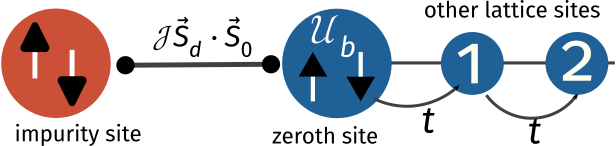
\includegraphics[height=0.07\textheight]{universal-theory.pdf}
	\hspace*{\fill}
	
\includegraphics[height=0.07\textheight]{two-site.pdf}
	\hspace*{\fill}
	\caption{{\it Left:} Schematic 1D construction of universal theory for the metal-insulator transition, obtained by integrating out the charge states of the impurity near the transition. {\it Right:} Zero bandwidth limit of the low-energy effective Hamiltonian for \(r\) between \(r_{c1}\) and \(r_{c2}\) (second row in table~\eqref{phases-table}). The bath is reduced to just a single degree of freedom - the zeroth site that is directly coupled to the impurity site.}
	\label{universal-theory}
\end{figure}

Indeed, the local correlation $\mathcal{U}_b$ encourages entanglement between the sites of the bath and makes the formation of the impurity-bath singlet difficult. In other words, the \(\mathcal{J}-\mathcal{U}_b\) model displays the destabilisation of the singlet by redistributing the entanglement from the impurity+bath system to purely within the bath (see left panel of Fig.~\eqref{twosite-spectrum}). Given the simplicity of these arguments, 
our analysis makes the case that local pairing fluctuations of the bath in eq.~\eqref{universal} offer a universal mechanism by which to frustrate the Kondo effect and lead thereby to an impurity transition that is the local counterpart of the Mott MIT obtained by auxiliary model approaches such as DMFT. We note that similar conclusions were reached in Refs.\cite{si_kotliar_1993,kotliarsi_1993,kotliar_1996} for the emergence of non-Fermi liquid phases at critical points in the mixed valence regime of the periodic Anderson model.

Further insight into the destabilisation of the singlet can be obtained from a zero-bandwidth approximation of the bath. Under such an approximation, the IR effective Hamiltonian obtained 
from the RG flow (row 2 of Fig.~\eqref{phases-table} takes the form of a two-site model with modified couplings (shown in the right panel of Fig.~\eqref{universal-theory}):
\begin{eqnarray}
\mathcal{\tilde J} \vec{S}_d\cdot\vec{S}_0 - \frac{1}{2}\mathcal{\tilde U}_b\left(\hat n_{0 \uparrow} - \hat n_{0 \downarrow}\right)^2 \label{zero-bw-pic}~.
\end{eqnarray}
The spectrum of this model is shown in the right panel of Fig.~\eqref{twosite-spectrum}. For \(|\mathcal{\tilde U}_b|/\mathcal{\tilde J} < 3/2\), the singlet ground-state (red) is separated from the excited local moment states (blue) by a gap of \(\frac{-3\mathcal{\tilde J}}{4} - \frac{\mathcal{\tilde U}_b}{2}\). As we tune \(r\) towards \(r_{c2}\), \(|\mathcal{\tilde U}_b|\) increases and the fixed point value \(\mathcal{\tilde J}\) decreases, leading to an overall reduction in the gap. At the critical point, the gap closes and the states become degenerate at zero energy; this is the equivalent of the quantum critical point at $r_{c2}$ of the full impurity model that was discussed earlier. We note that the vanishing of the energy of the metallic state was also observed by Brinkman and Rice from a Gutzwiller-type variational calculation of the Hubbard model at half-filling~\cite{brinkman_rice_1970}.

\begin{figure}[htpb]
	\includegraphics[width=0.41\textwidth]{mut-info-d0-01-across.pdf}
	\hspace*{\fill}
	\includegraphics[width=0.48\textwidth]{twosite_spectrum.pdf}
	\caption{{\it Left:} Very close to the transition, the mutual information \(I_2(d:0)\) (red curve) between impurity and the zeroth site reduces, while that between the zeroth and the first site (\(I_2(0:1)\), blue curve) increases, showing the redistribution of entanglement. {\it Right:} Spectrum of the zero bandwidth Hamiltonian of the right panel of Fig.~\eqref{universal-theory}. The blue line represents the local moment states at zero energy, while the red line represents the singlet state at an energy that continuously increases upon increasing \(r\).}
	\label{twosite-spectrum}
\end{figure}

\subsection{Local pairing and the destruction of Kondo screening} 
Very close to the transition at \(r_{c2}\), we find signatures of the breakdown of the Kondo cloud in terms of decaying impurity-zeroth site correlations (blue curve in the left panel of Fig.~\eqref{spin-charge-corr}) and enhanced intra-bath correlations. Remarkably, we find an {\it increase in pairing correlations} between the bath zeroth site and first site (red curve in the left panel of Fig.~\eqref{spin-charge-corr}). As discussed above, these are observed to be responsible for the destruction of the Kondo screening: spin and charge degrees of freedom are mutually exclusive, and the increased charge fluctuations on the bath zeroth site suppress the spin-flip scattering processes between the impurity and the zeroth site. We will show later that these fluctuations lead to the destruction of the local Fermi liquid excitations in our model, and replace them with non-Fermi local excitations in the neighbourhood of \(r_{c2}\).
We believe that the observed growth in non-local pairing correlations near the transition at \(r_{c2}\) is likely tied to a putative low-energy divergence of the local pairing susceptibility. A similar observation was made in Ref.\cite{si_kotliar_1993} from an auxiliary model-based analysis of a hole-doped extended Hubbard model in infinite dimensions that is pertinent to the physics of the heavy fermions. Similar to the conclusions of Ref.\cite{si_kotliar_1993}, we expect the pairing fluctuations of the bath to become dominant upon tuning the e-SIAM away from half-filling, signalling an instability towards a superconducting state.

\begin{figure}[!htpb]
	\centering
	$\vcenter{\hbox{\includegraphics[width=0.43\textwidth]{rc2-spin-charge-corr.pdf}}}$
	\hspace*{\fill}
	$\vcenter{\hbox{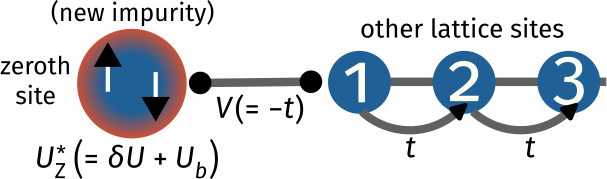
\includegraphics[width=0.45\textwidth]{decouple-impurity.pdf}}}$
	\caption{{\it Left:} Spin-flip correlation between the impurity and the bath (blue), and charge isospin-flip correlation between the bath zeroth and first sites (red), both as a function of the tuning parameter \(r\), very close to the transition. The operators are defined as \(S_i^+ = c^\dagger_{i \uparrow}c_{i \downarrow}\) and \(C_i^+ = c^\dagger_{i \uparrow}c^\dagger_{i \downarrow}\). {\it Right:} New effective SIAM Hamiltonian generated upon integrating out the coupling between the impurity and the bath zeroth site. In the new SIAM, the zeroth site acts as the new impurity site with a renormalised on-site correlation \(U_Z^* = U_b + \delta U_Z^*\).}
	\label{spin-charge-corr}
\end{figure}

\subsection{Emergent self-consistency in the e-SIAM}

As is well-established, the DMFT self-consistency equation is equivalent to requiring that the impurity Greens function become equal to the local Greens function in the bath~\cite{georges1996}.
Such a condition is also used in the projective self-consistent technique of Moeller et al.~\cite{moeller_1995} for the states within the central Kondo resonance.
We will now show that our model displays a qualitatively similar emergent feature.
To proceed, by employing a one-step URG transformation, we integrate out the impurity site from the rest of the fixed-point Hamiltonian of eq.~\eqref{fixed-point-ham}.
The details are shown in Sec. 4 of the Supplementary Materials~\cite{supp_mat}. The essential idea is similar to that of the Schrieffer-Wolff transformation: removing the impurity-bath couplings \(J\) and \(V\) generates an additional repulsive correlation \(\delta U_z^* \) on the zeroth site. The new low-energy model \(H_\text{Z}\) is therefore an Anderson impurity model with a net local correlation \(U_\text{Z}^* = \delta U_Z^* + U_b\) on the zeroth site (which is now the ``new impurity site"), and a single-particle hybridisation \(V_\text{Z}^* = -t\) coupling with a conduction bath formed by the remaining sites. This new impurity model is depicted schematically in the right panel of Fig.~\eqref{spin-charge-corr}.
\begin{eqnarray}
	H_\text{Z}^*  = \underbrace{-\frac{1}{2}U_\text{Z}^*\left(\hat n_{0\uparrow} - \hat n_{0\downarrow}\right)^2}_\text{new impurity = \(0^\text{th}\) site} + \underbrace{V_\text{Z}^*\sum_{\left<j,0 \right>}\left(c^\dagger_{0\sigma}c_{j\sigma} + \text{h.c.}\right)}_\text{hopping between \(0^\text{th}\) site \& new bath} + \underbrace{(-t) \sum_{\left<i,j \right>}\left(c^\dagger_{i\sigma}c_{j\sigma} + \text{h.c.}\right)}_\text{K.E. of new bath}~.
\end{eqnarray}

Since, for \(r < r_{c2}\), the model always flows to strong coupling at low energies, the largest energy scales are \(J^*\) and \(V^*\). Using this, the effective correlation \(U_Z^*\) on the zeroth site can be expressed to leading order as
\begin{eqnarray}
	\label{new-imp-correlation}
	U_\text{Z}^* \simeq \frac{J^*}{4}\frac{1}{1 + 2\gamma} - V^* \frac{\gamma}{\gamma^2 - \frac{1}{4}},~ \text{ where }\gamma\equiv V^*/J^*~.
\end{eqnarray}
From \(r = 0\) to \(r = r_{c1}\), the factor \(\gamma\) decreases due to the gradual removal of single-particle hopping from the impurity site (irrelevance of \(V\)), leading to an increase in the correlation \(U_Z^*\). This is simply a restatement of the fact that the scattering processes that create the central impurity resonance induce a repulsive correlation on the bath zeroth site. The fact that we end up with a standard SIAM on the zeroth site once the impurity site has been integrated out means that the spectral function of this new impurity will again go undergo a sharpening of the central peak (and the appearance of the Hubbard sidebands) upon increasing the parameter $r$ of the original e-SIAM. This ensures that the impurity and zeroth site spectral functions look qualitatively similar up to \(r_{c1}\). One can now repeat iteratively this process - decoupling the zeroth site generates a standard SIAM with a repulsive correlation on the first site, and so on. The fact that excursions starting from any point along the bath can be described by a positive \(U\) SIAM is, therefore, the emergent self-consistency in our model. Similar indications of a correlated spectral function on lattice sites far away from the impurity were also observed in Ref.\cite{martin2019} from finite-U slave boson calculations of the SIAM. Beyond \(r_{c1}\), the irrelevance of \(V\) means that \(U_Z^*\) reduces to just \(J^*/4\). As \(r\) is now increased towards \(r_{c2}\), the correlation decreases because \(J\) is moving towards its critical point, indicating that the bath zeroth site is moving away from its local moment regime. This is another reflection of the increase in pairing fluctuations of the bath, as well as the lowering of spin-flip fluctuations between the impurity and the bath.

For \(r > r_{c2}\), the impurity site decouples from the bath in the impurity model. This impurity model can be promoted to a bulk model as follows. Recall that in the auxiliary model mapping, any lattice site \(\vec r_i\) of the bulk lattice can act as the impurity, and one can think of the impurity model with the impurity at \(\vec r_i\) as a representation of the excursion of an electron from any such site \(\vec r_i\) into the rest of the bath. When all such impurity models undergo the transition at \(r = r_{c2}\) simultaneously, the result is the decoupling of all sites from their respective baths and a paramagnetic bulk insulator is obtained.

\section{Coexistence of local metallic and insulating phases in the e-SIAM}
\label{dmft}

The DMFT solution of the Hubbard model on the Bethe lattice exhibits a coexistence region of metallic and insulating solutions between two spinodal lines \(U_{c1}(T)\) and \(U_{c2}(T)\)~\cite{georges1996}, with the metallic solution having lower internal energy and the insulating solution being a metastable state at a higher energy~\cite{moeller_1995,georges1996,bulla_1999,georges_2004_dmft,georges_krauth_1993}.
The \(T=0\) transition is observed to be second order in nature and occurs through a merging of the metallic and insulating solutions at \(U_{c2}\)~\cite{rozenberg_1994_zerotemp,moeller_1995}. On the other hand, at $T>0$, the MIT happens along the first-order line \(U_c(T) \left(U_{c1} < U_c <U_{c2} \right)\) where the free energies of the two solutions become equal, and the two spinodal lines merge into a second order critical point at a sufficiently high temperature \(T_c\).  
We will now show that our Hamiltonian-based approach gives a clear zero temperature picture of various aspects that can lead to the emergence of the metal-insulator coexistence at $T>0$.

\subsection{Excited state quantum phase transition at \(r_{c1}\): the Mott-Hubbard scenario}

We have already discussed in detail the nature of the phase transition at \(r_{c2}\): the zero-bandwidth picture provided (around eq.~\eqref{zero-bw-pic}) shows the merging of the metallic and insulating solutions at that point, enabling identification of \(r_{c2}\) with the $T=0$ continuous phase transition observed at \(U_{c2}\) in the DMFT phase diagram. The focus of this subsection is the physics of the other important point \(r_{c1}\). As has been mentioned before, this point marks the RG irrelevance of the single-particle hybridisation amplitude \(V\), and leads to the exclusion of the charge states from the ground-state (see left panel of Fig.~\eqref{spec_func}). This exclusion means that there is now one fewer scattering channel by which the impurity electron can hybridise with the bath. In turn, this leads to a {\it partial localisation of the impurity}, and can be thought of as the first step towards the more complete localisation that occurs at \(r_{c2}\).

Apart from the change in the ground state, the physics at \(r_{c1}\) also involves a phase transition in certain excited states of the spectrum. To expose this, we consider the following states in the zero-bandwidth spectrum of the impurity model given in eq.~\eqref{GIAM-ham}:
\begin{equation}\begin{aligned}
	\label{esqpt-1}
	\ket{1,\sigma,\pm} &= \alpha_\pm \ket{\sigma_d}\ket{0_0} \mp \sqrt{1 - \alpha_\pm^2}\ket{0_d}\ket{\sigma_0}, ~\ket{3,\sigma,\pm} = \alpha_\pm \ket{\sigma_d}\ket{2_0} \mp \sqrt{1 - \alpha_\pm^2}\ket{2_d}\ket{\sigma_0} ~,\\
	E_+ &= -\frac{U_0}{4} + \sqrt{V_0^2 + \frac{U_0^2}{16}}, ~~E_- = -\frac{U_\text{im}}{4} - \sqrt{V_{\text{im}}^2 + \frac{U_{\text{im}}^2}{16}},\\
	\alpha_+(U_0,V_0) &= \frac{V_0}{\sqrt{V_0^2 + \left(E_+ + \frac{U_0}{2}\right)^2 }}, ~ ~\alpha_- = \frac{E_- + \frac{U_\text{im}}{2}}{\sqrt{V_\text{im}^2 + \left(E_- + \frac{U_\text{im}}{2}\right)^2 }}~.
\end{aligned}\end{equation}
where \(\left(\sigma=\uparrow,\downarrow\right)\) and \(E_\pm\) is the energy of the states \(\ket{1(3),\sigma,\pm}\) and the subscripts $d$ and $0$ refer to the impurity and bath zeroth site respectively. The states \(\ket{1(3),\sigma,+}\) are high-energy states, so their energy \(E_+\) and coefficient \(\alpha_+\) involve the bare single-particle hybridisation \(V_0\) and impurity on-site repulsion $U_{0}$. On the other hand, the other states \(\ket{1(3),\sigma,-}\) are closer to the IR energy scale and involve renormalised intermediate-scale couplings \(V_\text{im}\) and $U_{\text{im}}$. 
Both \(E_+\) and \(E_-\) are four-fold degenerate because of the SU(2) spin \((\uparrow \leftrightarrow \downarrow)\) and particle-hole \((\ket{0} \leftrightarrow \ket{2})\) symmetries. For example, the degenerate subspace corresponding to \(E_+\) is the set of states \(\left\{\ket{1,\uparrow,+}, \ket{1,\downarrow,+}, \ket{3,\uparrow,+}, \ket{3,\downarrow,+}\right\}\). 

All these states are in general delocalised - they involve the impurity hybridising with the bath via \(V\). At \(r = r_{c1}\), however, the coupling \(V\) becomes irrelevant and \(V_\text{im} \to 0\), so that the coefficient \(\alpha_-\) of the low-energy state becomes unity beyond that point. The low-energy states \(\ket{1(3),\sigma,-}\) thus become localised at \(r_{c1}\) and give rise to a set of excited and {\it degenerate local moment states}, i.e., $\alpha_- \to 0$ as $r \to r_{c1}$ leads to
\begin{eqnarray}
\ket{1(3),\sigma,-} \to \begin{cases}
	\ket{\uparrow_d}\ket{0_0}, \ket{\downarrow_d}\ket{0_0}\\
	\ket{\uparrow_d}\ket{2_0}, \ket{\downarrow_d}\ket{2_0}\\
\end{cases}~.
\end{eqnarray}
The other coefficient \(\alpha_+\) remains non-zero because, as mentioned earlier, \(V\) is non-zero in the UV scales of the RG flow. As a result, the high-energy states \(\ket{1(3),\sigma,+}\) remain delocalised, and are separated from the localised states by an energy-scale
\begin{eqnarray}
\lim_{r \to r_{c1}^-} \left(E_+ - E_-\right) &\simeq & \sqrt{V_0^2 + \left(\frac{U_0}{4}\right)^2} + \sqrt{V_{\text{im}}^2 + \left(\frac{U_{\text{im}}}{4}\right)^2} + \frac{U_{\text{im}}-U_0}{4}~.
\end{eqnarray}
This is shown schematically in the left panel of Fig.~\eqref{esqpt-schematic}, and corresponds to the preformed gap in the zero mode spectrum. The point \(r_{c1}\) therefore represents {\it a delocalisation-localisation excited state quantum phase transition} (ESQPT) where degenerate local moment states are emergent as excited states in the many-body spectrum. This localisation of the impurity at $r_{c1}$ is shown in the form of excited state mutual information in the right panel of Fig.~\eqref{esqpt-schematic}. This ESQPT acts as a precursor to the QPT at $r_{c2}$, where the local moment states become degenerate with the spin-singlet ground state. The local moment states are stabilised as ground states in the insulating phase for $r>r_{c2}$. 

\begin{figure}[htpb]
	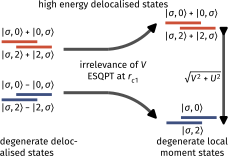
\includegraphics[width=0.43\textwidth]{ESQPT.pdf}
	\hspace*{\fill}
	\includegraphics[width=0.43\textwidth]{Uc1-mutinfo.pdf}
	\caption{{\it Left:} Evolution of the excited states mentioned in Eqs.~\eqref{esqpt-1} as \(r\) is tuned through \(r_{c1}\). The high-energy states (red) retain their impurity-bath coupling, while their low-energy counterparts (blue) become disentangled and form a degenerate set of local moment states. The high-energy states allow delocalisation into the bath and lead to the broad Hubbard sidebands. {\it Right:} Variation of mutual information (MI) between various parties, across the ESQPT at \(r_{c1}\). The MI (red) between the impurity and the zeroth site vanishes at \(r_{c1}\), showing the localisation of the impurity. The same between the bath zeroth site and the next site becomes maximum at \(r_{c1}\). The MI between the impurity and the other sites (purple and gray) of the bath show an initial rise near \(r_{c1}\), indicating that entanglement is becoming long-ranged near the ESQPT.}
	\label{esqpt-schematic}
\end{figure}

\subsection{Theory for the charge excitations in the Hubbard sidebands}
Beyond \(r_{c1}\), excitations into {\it the local moment states \(\ket{1,\sigma,-}\) and \(\ket{3,\sigma,-}\) reside at the edge of the central peak} in the impurity spectral function (purple curve in the right panel of Fig.\eqref{spec_func}) but provide no spectral weight due to the lack of electron mobility. This explains the development of a preformed gap in the impurity spectral function. That these local moment states have to reside at the edge of the central peak becomes clear when we note that as the width of the central peak shrinks continuously, the local moment states must also recede towards zero frequency and finally replace the zero frequency peak at \(r = r_{c2}\) in order to give rise to the insulating local moment phase for \(r > r_{c2}\). On the other hand, the {\it still-delocalised high-energy states \(\ket{1,\sigma,+}\) and \(\ket{3,\sigma,+}\) are pushed into the Hubbard sidebands}, and their hybridisation with the bath through \(V\) and \(t\) is responsible for the broadening of the sidebands. 

This isolation of the delocalised states into the sidebands means that charge delocalisation processes are now excluded from the physics at low energies. As accessing the sidebands involves excitations at exorbitantly high energy scales, such processes can only happen virtually and involve very short time scales. The central Kondo resonance observed at low energies, therefore, does not support any charge delocalisation, and metallic excitations propagate only through spin-flip scattering processes of the impurity. This reveals that the Mott insulator comes about through a local binding of doublons and holons~\cite{Mott_1949,kohn1964theory,castellani_1979}. Closely related to this is the Mott-Hubbard scenario of the MIT, which is equivalent to our observation of the appearance of an optical gap in the spectrum after \(r_{c1}\).

The fact that the sidebands are broad indicates that there are gapless excitations propagating from the impurity site into the conduction bath, but whose energy lies outside the Mott gap. These can also be viewed as metallic excitations of the bath that are induced by the coupled impurity. In order to expose the nature of these excitations, we perform a calculation similar to the local Fermi liquid calculation of Nozières~\cite{nozieres1974fermi}. This involves considering the states at \(\omega \sim \pm U/2\) as the ground-states of the Hubbard sidebands, and then computing how excitations into the bath renormalise the ground-state subspace. Up to the second order in the hopping strength \(t\), the effective Hamiltonian for the excitations of the bath can be expressed as
\begin{eqnarray}
H_\text{eff}^{(2)} = \frac{4t^2(1 - \alpha_+^2)}{E_+ - E_\text{gs}}C_\text{tot}^z C_1^z - t\sum_{i >0,\sigma}\left(c^\dagger_{i\sigma}c_{i+1\sigma} + \text{h.c.}\right) ~,\label{hodoLFL}
\end{eqnarray}
where \(E_+\) and \(\alpha_+\) have been defined in eq.~\eqref{esqpt-1}, \(C_i^z\ket{2(0)} = +(-)\frac{1}{2}\ket{2(0)}\) is the z-component of the charge isospin operator at a particular site $i$, and \(\vec C_\text{tot} = \vec C_d + \vec C_0\) is the total isospin for the impurity and zeroth sites.
\(E_\text{gs} = U/2\) is the two-site energy of the ground-state subspace within the sideband.
These excitations are of the local Fermi liquid kind - the absence of any isospin-flip scattering term promotes the independent delocalisation of the doublon and holon states into the bath. The second-order effective Hamiltonian can therefore be written as the sum of two decoupled parts corresponding to holon and doublon propagation respectively, and suggesting adiabatic continuity with the \(U=0\) Hubbard model~\cite{hrk_1990_prl}. 

However, fourth-order corrections lead to the appearance of scattering processes that convert holon and doublons into one another, resulting in the local Fermi liquid becoming correlated
\begin{eqnarray}
	H_\text{eff}^{(4)} = \frac{\gamma^4 \alpha_+^2 \beta^2}{\left( 1 - \alpha_+^2 \right) \left( E_+^\prime - E_\text{gs} \right) } \left[- C_\text{tot}^z C_\text{tot}^2 C_1^z + \sqrt{2}\mathcal{P}_\text{tot}^{4}\left(C_0^+ - C_d^+\right)C_1^- + \text{h.c.}\right]~,\label{holonLFL}
\end{eqnarray}
where \(E_+^\prime = \frac{U}{4} - \frac{3J}{8} + \sqrt{4V^2 + \left(\frac{U}{4} + \frac{3J}{8}\right)^2}\) is the energy of the state containing the charge isospin triplet zero, and \(\beta = \frac{2V}{\sqrt{4V^2 + \left(U + 3J/4\right)^2}}\). \(\mathcal{P}^4_\text{tot}\) projects on to the \(n_d + n_0 = 4\) subspace.
The scattering processes in eq.~\eqref{holonLFL} are clearly non-Fermi liquid in nature as they allow the inter-conversion of the charge isospin eigenstates, and therefore reduce the lifetime of the quasiparticle excitations of the local Fermi liquid obtained in eq.~\eqref{holonLFL}. Additional details pertaining to the calculation of this effective Hamiltonian are present in Sec. 5 of the Supplementary Materials~\cite{supp_mat}.

\subsection{Zero temperature origin of critical fluctuations above the second order point}
\label{rc2-corrs}

\begin{figure}[htpb]
	\centering
	\includegraphics[width=0.45\textwidth]{Uc1-1p.pdf}\\
	\includegraphics[width=0.45\textwidth]{Uc1-spin-charge-01.pdf}
	\hspace*{\fill}
	\includegraphics[width=0.45\textwidth]{Uc1-spin-charge-02.pdf}
	\caption{{\it Top:} Variation of the one particle correlations in the state \(\ket{1,\sigma,-}\) between impurity and bath zeroth site(blue), as well as within the bath (red and violet). The former vanishes, depicting the excited state localisation transition at \(r_{c1}\). {\it Left:} Variation of the spin-flip (red) and charge isospin-flip (blue) correlations between impurity and bath, close to \(r_{c1}\). They both increase, indicating that the impurity is now less strongly coupled with the bath. {\it Right:} Variation of the spin-flip (red) and charge isospin-flip (blue) correlations between the zeroth and second sites of the bath, close to \(r_{c1}\). Both show an initial increase, leading to the propagation of relatively long-range correlations into the bath.}
	\label{Uc1-sc-02}
\end{figure}

Above the second order point \(r_c(T_c)\), the DMFT phase diagram shows a rapid crossover from the paramagnetic metallic solution to the paramagnetic insulating solution~\cite{georges1996,limelette_2003}. Remarkably, signatures of quantum critical scaling in this crossover region have been recently predicted from theoretical analyses~\cite{terletska_mott_2011,vucicevic_2013}, as well as detected experimentally in transport measurements of several organic compounds~\cite{Kagawa2005,Furukawa2015}. In Refs.\cite{terletska_mott_2011,vucicevic_2013}, this has been ascribed to the existence of a \textit{hidden quantum criticality} in the maximally frustrated $1/2$-filled Hubbard model on the Bethe lattice with infinite coordination number. In order to locate the zero temperature origin of these signatures of quantum criticality, we inspect carefully the quantum-mechanical fluctuations near the two important points \(r_{c1}\) and \(r_{c2}\) in our model.

Close to \(r_{c1}\), we compute correlations in the state \(\ket{1,\sigma,-}\).
As shown in the top panel of Fig.~\eqref{Uc1-sc-02}, we find that while the one-particle correlation between the impurity and the bath vanishes, the same between the zeroth and first sites of the bath picks up. Importantly, these correlations extend beyond the immediate neighbourhood of the impurity. This is observed in, for example, the one-particle correlation between the zeroth site and the second site (purple curve in the top panel of Fig.~\eqref{Uc1-sc-02}). Some other signatures of correlations in the bath are shown in Fig.~\eqref{Uc1-sc-02}: while the left panel displays increased spin-flip and charge isospin-flip correlations between the zeroth and first sites of the bath, a similar phenomenon is observed between the zeroth and second sites of the bath in the right panel. 
Our findings are consistent with the presence of scale-invariant solutions obtained from recent NRG-DMFT calculations ~\cite{Eisenlohr_2019} that correspond to the metastable insulating solutions in the coexistence region.

The growth of similar long-ranged correlations within the bath (and leading away from the immediate neighbourhood of the impurity) 
near \(r_{c2}\) as well.
We recall that correlations between the impurity and the zeroth site are observed to decrease (see left panel of Fig.\eqref{gstate-correlations}).
Instead, as shown in Fig.~\eqref{Uc2-ss}, non-trivial two-particle correlations arise between the impurity and bath zeroth sites with bath sites that are farther away.
The spreading of the spin-spin correlations shown in the left panel of Fig.~\eqref{Uc2-ss} indicates a ``stretching" of the Kondo singlet state prior to its destruction. We will show later that these enhanced correlations also result in a diverging quasiparticle mass at \(r_{c2}\), indicating a breakdown of the local Fermi liquid metal. Further, the right panel of Fig.~\eqref{Uc2-ss} indicates that longer-ranged pairing correlations develop between the bath zeroth site and bath sites farther away upon approaching the transition.

In general, within the metallic phase and away from \(r_{c1}\) or \(r_{c2}\), the impurity is strongly coupled to the bath zeroth site and the impurity-bath entanglement follows an area law characteristic of the local nature of the impurity problem. However, near the excited state and ground state transitions at \(r_{c1}\) or \(r_{c2}\) respectively, these results indicate a spreading of entanglement into the bath: more and more bath sites beyond the zeroth site get correlated with the impurity site as the ESQPT or the QCP is approached. This is corroborated in Fig. 3 of the Supplementary Materials~\cite{supp_mat}.
This suggests a significant enhancement of the entanglement beyond the area law and is consistent with the critical quantum fluctuations observed in the various two-particle correlations. 

The results of this subsection indicate that it might be possible to experimentally detect the signatures of such critical quantum fluctuations around the spinodals of the DMFT phase diagram even at \(T > 0\). We note that signatures of second-order criticality have been indeed observed recently in vanadium sesquioxide, in the form of critical slowing down and critical opalescence~\cite{satyaki_2020_PRL}. It is, therefore, tempting to speculate that these signatures arise from the presence of critical quantum fluctuations.

\begin{figure}[htpb]
	\includegraphics[width=0.45\textwidth]{rc2-spinspin-corr-di.pdf}
	\hspace*{\fill}
	\includegraphics[width=0.45\textwidth]{rc2-charge-flip-corr-0i.pdf}
	\caption{{\it Left:} Variation of the spin-spin correlations between the impurity and bath sites 1 through 4, close to \(r_{c2}\). They show an increase, revealing the distribution of entanglement into the bath. {\it Right:} Variation of pairing correlations within the bath. These correlations show an increase, because of the weakening of the Kondo singlet.}
	\label{Uc2-ss}
\end{figure}

\section{Non-Fermi liquid signatures at the MIT}
\label{excitations}

\subsection{Death of the local Fermi liquid: the Brinkman-Rice scenario}

The low-lying metallic excitations of the bath can be obtained by considering the singlet ground-state of the model (of energy \(\sim -3\mathcal{\tilde J}/4\)) in the metallic phase, and then studying the effect of an electron hopping term (with coupling \(t\)) between the singlet and the rest of the bath as a perturbation (see left panel of Fig.~\eqref{lorentzian}). Such a strong-coupling expansion in powers of \(t^2/\mathcal{\tilde J}\) leads to the usual local Fermi liquid effective Hamiltonian in the Kondo model~\cite{nozieres1974fermi,wilson1975,Noz_blandin_1980,anirban_kondo}:
\begin{eqnarray}
	\label{lfl-ham}
	H_\text{LFL} = \mathcal{F} \hat n_{1 \uparrow} \hat n_{1 \downarrow} + H_\text{KE}~, ~ ~ \mathcal{F} \sim t^4 / \mathcal{\tilde J}^3~,
\end{eqnarray}
where \(\hat n_{1 \sigma}\) are the number operators for the first site (site adjacent to the zeroth site of the conduction bath), \(H_\text{KE}\) is the kinetic energy arising from the nearest-neighbour hopping among all sites in the bath apart from the zeroth site, and \(\mathcal{F}\) is the local Fermi liquid correlation strength. The Kondo singlet (formed between the impurity spin and the bath zeroth site) has decoupled from the rest of the lattice, and eq.~\eqref{lfl-ham} describes the effective Hamiltonian for the rest of the bath beyond the zeroth site. 

Following an identical approach, we find that the effective Hamiltonian for the low-lying excitations in the metallic phase is given by
\begin{eqnarray}
	H_\text{LFL} = \mathcal{F}\left[\hat n_{1 \uparrow} \hat n_{1 \downarrow} + \left(1 - \hat n_{1 \uparrow}\right) \left(1 - \hat n_{1 \downarrow}\right) \right] + H_\text{KE},\quad \text{ where }\mathcal{F} = \frac{2t^4}{\mathcal{\tilde J}\left(3\mathcal{\tilde J}/4 + \mathcal{\tilde U}_b\right)^2}~.
\end{eqnarray}
We note that for our extended SIAM, the local Fermi liquid correlation \(\mathcal{F}\) diverges as the transition is approached at \(3\mathcal{\tilde J}/4 + \mathcal{\tilde U}_b \to 0\). The divergence of \(\mathcal{F}\) leads to the divergence of the renormalised mass of the quasiparticles, and can also be obtained from a Gutzwiller variational calculation as shown by Brinkman and Rice~\cite{brinkman_rice_1970}. This shows the breakdown of perturbation theory and is indicative of the fact that the ground state is about to change at the metal-insulator transition.

The death of the local Fermi liquid is also seen from the vanishing of the dynamically generated low-energy Kondo screening scale \(T_K\). Towards obtaining $T_K$ close to the transition, we follow the approach used by Moeller et al. 1995~\cite{moeller_1995} and Held et al. 2013~\cite{held_2013}. Near the transition, they obtained a Kondo model from the SIAM by applying a Schrieffer-Wolff transition that removes the charge fluctuations of the impurity site and retains the physics of only the Kondo coupling \(J\). This amounts to removing the side peaks from the impurity spectral function and focusing on the low-energy central peak (right panel of Fig.~\eqref{lorentzian}). Held et al. then integrated the RG equation for this Kondo model by using a Lorentzian DOS \(\rho(D)\) in the bath: \(\rho(D) = \frac{\rho_0 \Gamma^2}{D^2 + \Gamma^2}\).
\begin{figure}[htpb]
	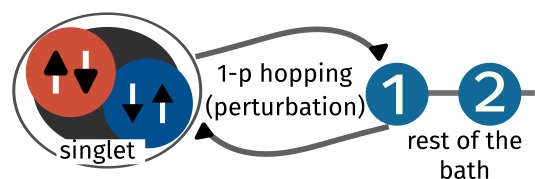
\includegraphics[width=0.45\textwidth]{perturbation.pdf}
	\hspace*{\fill}
	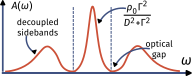
\includegraphics[width=0.4\textwidth]{lorentzian.pdf}
	\caption{{\it Left:} Setup for obtaining the low-energy excitations above the strong-coupling ground state. The effects of the rest of the bath is included by treating the hopping between the zeroth site (blue sphere on the left) and the first site (sphere labelled 1) as a perturbation on top of the singlet ground state formed by the impurity (red sphere) and the zeroth site. {\it Right:} At \(r_{c1}\), the Hubbard sidebands have become isolated from the central peak in the local spectral function because of the finite optical gap. Removing the UV excitations that couple the low-energy and high-energy bands then leads to a theory of the Kondo model with a Lorentzian DOS.}
	\label{lorentzian}
\end{figure}
This is motivated by the fact that the central peak of the impurity spectral function is a Lorentzian, and the bath becomes equivalent to the impurity site under self-consistency.

We implement the same approach on the e-SIAM, such that the Schrieffer-Wolff transformation leads to a \(J-U_b\) model with a Lorentzian electronic DOS in the bath. The expression of the Kondo temperature for such a system has been derived in Sec. 6 of the Supplementary Materials~\cite{supp_mat}. Very close to the transition, we have \(r \to 0.25^{-}\), and the Kondo temperature is given by
\begin{eqnarray}
	T_K = \frac{D_0}{k_B} \exp\left[-\frac{\ln\left( r_{c2} - r \right)}{4 U_b \rho_0}\right]~,
\end{eqnarray}
where \(r_{c2} = 0.25\) and \(D_0\) is the bare bandwidth. Note that the pre-factor of the logarithm is positive as \(U_b\) is negative: \(-4U_b\rho_0 = |4U_b \rho_0|\). As we approach the transition, the parameter \(r\) takes the limit \(r \to r_{c2}^-\), and the Kondo temperature scale vanishes:
\begin{eqnarray}
	\lim_{r \to r_{c2}^-} T_K = \frac{D_0}{k_B} \lim_{r \to r_{c2}^-}\left(r_{c2} - r\right)^{4|U_b\rho_0|} \to 0~.
\end{eqnarray}
Following the renormalised perturbation theory approach of Hewson~\cite{hewson1993,coleman2015}, the imaginary part of the self-energy of the local Fermi liquid quasiparticles is given by
\begin{eqnarray}
	\text{Im}\left[\Sigma(\omega)\right] \sim \frac{\mathcal{F}^2}{D_{0}} \frac{\omega^2}{T_{K}^{2}}~, \label{sigma_rc2}
\end{eqnarray}
while the quasiparticle residue is given by \(Z \sim T_K\). The divergence of \(\text{Im}\left[\Sigma(\omega)\right]\) at the transition and the vanishing of \(T_K\) and the quasiparticle residue are important indicators of the loss of the local Fermi liquid excitations and the breakdown of Kondo screening.

The vanishing of the Kondo temperature scale also leads to the divergence of thermodynamic quantities such as the impurity contribution to local spin susceptibility \(\chi_\text{imp}\) and the specific heat coefficient \(\gamma_\text{imp}\). As the low-energy theory is a local Fermi liquid, \(\chi_\text{imp}\) and \(\gamma_\text{imp}\) retain their Fermi liquid forms but involve the highly renormalised Kondo temperature scale~\cite{wilson1975,hewson_1993_prl}:
\begin{eqnarray}
	\chi_\text{imp} = \frac{w}{4k_B T_K}, \quad\lim_{r \to r_{c2}^-}\chi_\text{imp} = \frac{w}{4k_B}\left(r_{c2} - r\right)^{-4|U_b\rho_0|}, \nonumber\\
	\gamma_\text{imp} = \frac{\pi^2 k_B^2 w}{6 T_K}, \quad \lim_{r \to r_{c2}^-}\gamma_\text{imp} = \frac{\pi^2 k_B^2 w}{6}\left(r_{c2} - r\right)^{-4|U_b\rho_0|}~,
\end{eqnarray}
where \(w \sim 0.4128\) is the Wilson number for the Kondo model~\cite{wilson1975,anirban_kondo}. These results also show that the ratio of \(\chi_\text{imp}\) and \(\gamma_\text{imp}\), referred to as the Wilson ratio \(R \equiv \frac{4\pi^2 k_B^2 \chi_\text{imp}}{3 \gamma_\text{imp}}\), remains pinned at the single-channel Kondo value of \(R_\text{LFL} = 2\) for \(r \to r_{c2}-\). This shows that the low-frequency Landau quasiparticles are able to survive until very close to the QCP. As we will show in the next subsection, the metallic excitations precisely at the QCP acquire non-Fermi liquid character and involve additional correlations between holons and doublons. These additional correlations are expected to lead to an enhancement of the Wilson ratio. Evidence for this can be found in the DMFT calculation of a local Wilson ratio very close to the Brinkman-Rice transition, \(R_\text{loc} = 2.9 \pm 0.2\)~\cite{georges1996}.

\subsection{Emergence of non-Fermi liquid excitations at the transition}

In order to obtain an effective Hamiltonian for the excitations precisely at the critical point \(r=1/4\), we first note that the ground-state subspace of the zero bandwidth $J-U_{b}$ effective model (eq.~\eqref{zero-bw-pic}) becomes degenerate at this point:
\begin{eqnarray}
\frac{1}{\sqrt 2}\left(\ket{\uparrow}_d\ket{\downarrow}_0 - \ket{\downarrow}_d\ket{\uparrow}_0\right)~,~ \ket{\sigma}_d\ket{0}_0~,~\ket{\sigma}\ket{2}_0~,~~~ (\sigma=\uparrow,\downarrow)~,
\end{eqnarray}
with all the states lying at zero energy. Here, the first ket (with subscript \(d\)) represents the impurity spin configuration while the second ket (with subscript \(0\)) represents the configuration of the bath zeroth site). We now diagonalise these states in the presence of the electron hopping \(t\) into the rest of the conduction bath, and obtain the effective Hamiltonian for the low-lying excitations mediated by \(t\). This is described in detail in Sec. 7 of the Supplementary Materials~\cite{supp_mat}. We note that the ground state is four-fold degenerate at energy \(-t\) in the presence of the hopping, and comprises the following states:
\begin{eqnarray}
	\label{degenerate-nfl}
	\ket{N_\text{tot}=2,S^z_\text{tot}=0}~,~\ket{N_\text{tot}=4,S^z_\text{tot}=0}~, ~\ket{N_\text{tot}=3,S^z_\text{tot}=\frac{1}{2}}~,~\ket{N_\text{tot}=3,S^z_\text{tot}=-\frac{1}{2}}~,
\end{eqnarray}
where \(N_\text{tot} = \hat n_d + \hat n_0 + \hat n_1\) and \(S^z_\text{tot} = S^z_d + S^z_0 + S^z_1\) are the total number operator and total magnetisation operator respectively for the impurity, bath zeroth and first sites taken together. It is worth observing that
\begin{itemize}
	\item the presence of the unscreened states \(\ket{N_\text{tot}=3,S^z_\text{tot}=\pm\frac{1}{2}}\) in the ground-state subspace is a result of the inexact screening at the critical point, and
	\item the presence of a degenerate ground-state manifold indicates that these excitations of the bath will likely be of the non-Fermi liquid (NFL) kind~\cite{varma2002singular,si_kotliar_1993,Kotliar_1993}.
\end{itemize}
The precise form of the effective Hamiltonian for this non-Fermi liquid, as well as the behaviour of various correlation functions, is obtained by considering the ground-state manifold in conjunction with the excited states at energy \(-t\). 

Since the total Hamiltonian conserves the total spin \(S_\text{tot}^z\), the effective Hamiltonian separates into two sectors, \(S_\text{tot}^z = 0\) and \(|S_\text{tot}^z| = \frac{1}{2}\). Detailed calculations on obtaining this effective Hamiltonian from the RG fixed point theory are shown in Sec. 7 of the Supplementary Materials~\cite{supp_mat}. In order to highlight certain distinct features, we present simplified effective Hamiltonians only for the \(S_\text{tot}^z = 0\) and \(S_\text{tot}^z = \frac{1}{2}\) sectors. We first take a look at the \(S^z_\text{tot}=0\) sector:
\begin{eqnarray}
	H_\text{eff}^{S^z_\text{tot}=0} = t\vec{S}_d\cdot\left(\vec{\mathcal{S}}_{1,-} + \vec{\mathcal{S}}_{3,-}\right)
	\label{unscreened_sector1}~.
\end{eqnarray}
The effective spin-1/2 ladder operators \(\vec{\mathcal{S}}_{1,\pm}\) act on the positive and negative parity sectors (labelled by $\pm$) of the \(\hat n_0 + \hat n_1 = 1\) subspace spanned by the states
\begin{eqnarray}
	\ket{\Uparrow}_{1,\pm} = \ket{\uparrow}_0\ket{0}_1 \pm \ket{0}_0\ket{\uparrow}_1, \quad \ket{\Downarrow}_{1,\pm} = \ket{\downarrow}_0\ket{0}_1 \pm \ket{0}_0\ket{\downarrow}_1~,
\end{eqnarray}
leading to a Pauli matrix representation of $\vec{\mathcal{S}}_{1,\pm}$ in that basis.
The Pauli matrix operators \(\vec{\mathcal{S}}_{3,\pm}\) similarly act on the \(\hat n_0 + \hat n_1 = 3\) subspace spanned by the states \(\ket{\Uparrow}_{3,\pm} = \ket{\uparrow}_0\ket{2}_1 \pm \ket{2}_0\ket{\uparrow}_1\) and \(\ket{\Downarrow}_{3,\pm} = \ket{\downarrow}_0\ket{2}_1 \pm \ket{2}_0\ket{\downarrow}_1\), obtained by applying the transformation \(\ket{0} \to {2}\) on the \(\hat n_0 + \hat n_1 = 1\) counterparts. 
We now point out two interesting features of this simplified effective Hamiltonian in eq.~\eqref{unscreened_sector1}.
\begin{itemize}
	\item The fact that the impurity is now interacting with emergent spins \(\vec{\mathcal{S}}_1\) and \(\vec{\mathcal{S}}_3\) that span over two lattice sites (0 and 1) instead of just the zeroth site indicates that the entanglement between the impurity and bath is now extended beyond the bath zeroth site, and that {\it the singlet is being stretched}. 
	\item The presence of two spins that are trying to simultaneously screen the impurity spin introduces frustration in the dynamics of the impurity. This is reminiscent of the 2-channel Kondo effect, and the connection is made more precise in the concluding section of our work. 
\end{itemize}
Both these features are precursors to the ultimate and complete destruction of screening in the local moment regime, and reflect the fact that the impurity-bath system {\it is now in an over-screened state}.

We now focus on the effective Hamiltonian of the \(S^z_\text{tot} \neq 0\) subspace:
\begin{eqnarray}
	 H_\text{eff}^{S^z_\text{tot}\neq 0} = -\frac{1}{2}t\left(S_d^- \mathcal{B}^+_\uparrow + \text{h.c.}\right) \label{unscreened_sector2}~.
\end{eqnarray}
The Pauli matrix operators \(\mathcal{B}^+_\uparrow\) and \(\mathcal{B}^-_\uparrow\) flip between the doublet of states \(\ket{\uparrow}_0\ket{\uparrow}_1\) and \(\frac{1}{\sqrt 2}\left( \ket{2}_0\ket{0}_1 + \ket{0}_0\ket{2}_1 \right) \):
\begin{eqnarray}\label{andreev}
	\mathcal{B}^-_\uparrow\ket{\uparrow}_0\ket{\uparrow}_1 = \frac{1}{\sqrt 2}\left( \ket{2}_0\ket{0}_1 + \ket{0}_0\ket{2}_1 \right),\nonumber \\
	\mathcal{B}^+_\uparrow\frac{1}{\sqrt 2}\left( \ket{2}_0\ket{0}_1 + \ket{0}_0\ket{2}_1 \right) = \ket{\uparrow}_0\ket{\uparrow}_1~.
\end{eqnarray}
The structure of the effective Hamiltonian in eq.~\eqref{unscreened_sector2} leads to another drastic difference from the behaviour of the local Fermi liquid: it allows for the electrons to be ``Andreev scattered" into an orthogonal state by hopping from the first site into the zeroth site. This is easily seen by considering the scattering processes in eq.~\eqref{andreev}: a state \(\ket{\uparrow}_0\ket{\uparrow}_1\) (i.e., with site 1 in $\uparrow$ configuration) has a finite probability of being flipped into the \(\ket{\downarrow}_0\ket{2}_1\) state (i.e., with site 1 in the doublon configuration). {\it An incident electron \(c^\dagger_{1 \uparrow}\) can therefore emerge as a doublon \(c^\dagger_{1 \uparrow}c^\dagger_{1 \downarrow}\) or a hole \(c_{1 \uparrow}\) upon scattering from the zeroth site}. This is a direct consequence of the entanglement between the singlet and the first site at the critical point that was absent in the metallic regime of the e-SIAM. We note that similar orthogonal scattering processes also occur in a two-channel Kondo problem between effective pseudo-particles and pseudo-holes~\cite{von_delft_1998}.

At this point, it is worth noting that the polarised ground-state \(\ket{S_\text{tot}^z=\frac{1}{2}}\) can be written as an equal superposition of the singlet state \(\ket{\text{SS}}_{d0}\otimes\ket{\uparrow}_1\) and the local moment states \(\frac{1}{\sqrt 2}\left(\ket{\uparrow, 0, 2} - \ket{\uparrow, 2, 0}\right)\). This symmetry-broken ground state, along with its counterpart $\ket{S_\text{tot}^z=-\frac{1}{2}}$, act as a bridge between the ground states of the metallic and insulating phases. They are thus important in displaying the breakdown of the Kondo cloud at the QCP, and the consequences arising from it. We will hence consider these states in the next subsection and demonstrate some exotic non-Fermi liquid properties of these states, e.g., inexact screening of the impurity, fractional impurity magnetisation and fractional impurity entanglement entropy.

Finally, by mapping the quantum impurity problem of the e-SIAM onto that of a classical Coulomb gas~\cite{anderson1969exact,si_kotliar_1993}, it can be shown that the local self-energies \(\Sigma_{dd}(\omega)\) and \(\Sigma_{00}(\omega)\) of the impurity and zeroth sites respectively and certain two-particle correlation functions have power-law behaviours in the frequency domain:
\begin{eqnarray}\label{exponents}
	\text{Re}\left[\Sigma_{dd}\right](\omega) \sim |\omega|^{\gamma_{dd}}, ~ ~\text{Re}\left[\Sigma_{00}\right](\omega) \sim |\omega|^{\gamma_{00}}~,\\
\left<S_d^+\right> \sim |\omega|^{(\alpha_1 - 1)/2}, ~ ~\left<c^\dagger_{0 \uparrow} c^\dagger_{ 0\downarrow}\right> \sim |\omega|^{(\alpha_3 - 1)/2}~.
\end{eqnarray}
The precise forms of the exponents in terms of the conduction electron scattering phase shifts, as well as several other technical details of the calculation, are provided in Sec. 8 of the Supplementary Materials~\cite{supp_mat}. While the various exponents are found to be non-universal functions of the fixed point value of $J$ and the coupling $U_{b}$ for $r\to r_{c2}-$, we argue in subsection \eqref{excess} that they assume universal values precisely at the QCP ($r=r_{c2}$). The algebraic behaviour of these local correlations
is reminiscent of critical behaviour ascribed to the class of local quantum criticality~\cite{Coleman_Si_2001,Si2001}. 


\subsection{Impurity magnetisation and entanglement entropy}
More indications of non-Fermi liquid behaviour at the QCP is obtained from a calculation of the impurity magnetisation and the impurity entanglement entropy (\(S_\text{EE}(d)\)) (shown in Sec. 9 of the Supplementary Materials~\cite{supp_mat}) for the symmetry-broken states \(\ket{S_\text{tot}^z = \sigma/2}\). This 
leads to a fractional entanglement entropy (in units of \(\log 2\)) for each of the two states:
\begin{eqnarray}
	\rho_\text{imp} &=& \begin{pmatrix} \frac{1}{2} + m_\text{imp}^z & 0 \\ 0 & \frac{1}{2} - m_\text{imp}^z \end{pmatrix} = \begin{pmatrix} \frac{3}{4} & 0 \\ 0 & \frac{1}{4} \end{pmatrix}~,\nonumber\\ 
	S_\text{EE}(d) &=& -\text{Tr}\left(\rho_\text{imp} \ln \rho_\text{imp}\right) \simeq 0.81 \log 2~,
\end{eqnarray}
where the impurity magnetisation \(m_\text{imp}^z\) takes the value \(m_\text{imp}^z = 1/4\) at the QCP (i.e., half the value for a local moment).
Further, \(S_\text{EE}(d)\) can be written in terms of an effective impurity degeneracy \(g_\text{imp}\), which we define using the impurity magnetisation: \(g_\text{imp} \equiv 1 + 2|m_\text{imp}^z|\), such that it takes the expected values of 1 and 2 in the local Fermi liquid and local moment phases (with \(m_\text{imp}^z\) having values 0 and \(\frac{1}{2}\) respectively). The effective degeneracy in the polarised subspace \(S_\text{tot}^z = \pm 1/2\) at the QCP then turns out to be \(3/2\), which is half-way between a unique state and a doublet. This corresponds to partial screening of the impurity degrees of freedom at the QCP, in contrast to complete screening in the metallic phase (\(g_\text{imp} = 1\)) and the absence of screening in the insulating phase (\(g_\text{imp} = 2\)).

In Sec. 9 of the Supplementary Materials~\cite{supp_mat}, we show that the incomplete magnetisation (and hence the fractional value of \(S_\text{EE}\)) arises from the mixing of the local Fermi liquid ground-state \(\ket{\phi} = \otimes_{k <= k_F} \ket{k \uparrow}\ket{k \downarrow}\) and the gapless excitations above it, \(\ket{e}_\sigma = e^\dagger_\sigma \ket{\phi}, e \equiv \sum_{k \in FS} c^\dagger_{k\sigma}\), leading to the decay of the local Fermi liquid quasiparticles~\cite{varma2002singular}. This is captured by the modified ground-state \(\ket{-}\) and lowest-lying excited states \(\ket{+}\) at the QCP:
\begin{eqnarray}\label{new-ground-state}
	\ket{\pm} = \frac{1}{\sqrt 2}\left(\ket{SS}\otimes\ket{e}_\sigma \pm \ket{LM}_\sigma\otimes\ket{\phi}\right)~.
\end{eqnarray}
The spin-singlet state \(\ket{SS} \sim \sum_\sigma \sigma\ket{\sigma}_d\ket{\bar\sigma}_0\) and the local moment state \(\ket{LM}_\sigma = \ket{\sigma}_d \ket{2}_0\) represent the configurations of the impurity and the bath zeroth sites. Such a ground-state \(\ket{-}\) should be contrasted with the local Fermi liquid ground-state \(\ket{SS}\otimes\ket{\phi}\) that is stable in the metallic phase for \(r_{c1} < r < r_{c2}\). This change in the ground-state manifests in the vanishing of the quasiparticle residue of the local Fermi liquid excitations: \(Z = |\braket{+ | e^\dagger_{\sigma} | -}|^2 = |\bra{+} \left(\ket{LM}_\sigma\otimes \ket{e}_\sigma\right)|^2 = 0\), consistent with the orthogonality catastrophe~\cite{anderson1967infrared} described below eq.~\eqref{sigma_rc2}.
As the local Fermi liquid quasiparticles are rendered unstable, they are replaced by stable composite three-site excitations of the form, \(S_d^- c_{0 \bar\sigma} e^\dagger_\sigma\). This is further reflected in the fact that the corresponding residue for such three-site composite excitation is non-zero at the QCP: \(|\braket{+|S_d^- c_{0 \bar\sigma} e^\dagger_\sigma|-}|^2 > 0\).

\subsection{Friedel scattering phase shift and fractional excess charge}\label{excess}
The orthogonality catastrophe faced by the infrared excitations of the conduction bath at the QCP points towards the presence of an ``unrenormalised" phase shift~\cite{anderson1990} of the scattering \(k-\)states. Indeed, using the Friedel sum rule~\cite{friedel_1956,langer1961friedel,langreth1966}, we obtain a \(\pi/2\) phase shift for the extended states at the Fermi surface for the QCP, which is only half the unitary limit. This can be seen by recalling that the ground state in eq.~\eqref{new-ground-state} is an equal admixture of a decoupled local moment state and a singlet state. Through the singlet state, the impurity contributes an excess charge of unity to the Fermi surface of the conduction bath (because of the presence of gapless spin-flip fluctuations). The local moment state does not contribute any excess charge, because the impurity is decoupled from the bath. The net excess charge then comes out to be \(n_\text{exc} = \frac{1}{2}\left( 1 + 0 \right) = \frac{1}{2}\). From the Friedel sum rule, the phase shift at the fixed point is \(\delta^* = \pi n_\text{exc} = \pi /2\), as mentioned above. Expectedly, \(n_\text{exc}\) is zero in the local moment phase. Also, as the exponents of the algebraic form for the local quantities shown in eq.~\eqref{exponents} are functions of the scattering phase shift, we find that these exponents take universal values precisely at the QCP.

The values of the excess charge at the QCP and in the local moment phase lead to important corollaries. Firstly, the jump in the excess charge by unity in going from \(r < r_{c2}\) to \(r > r_{c2}\) is in fact a reduction in the Luttinger volume \(V_L\) of the conduction bath~\cite{luttinger1960fermi,martin_1982}. \(V_L\) counts the number of extended states present at and below the Fermi volume, and corresponds to a  topological quantum number~\cite{oshikawa2000topological,seki2017topological,Heath2020,anirbanurg1}. Since the excess charge \(n_\text{exc}\) calculated above is simply the impurity contribution to \(V_L\) at the Fermi surface, the difference in the excess charge across the transition implies that the two phases acquire different values for the invariant \(V_L\). Thus, $n_\text{exc}$ tracks the change ($\Delta V_{L}$) in the Luttinger volume, and the transition is topological in nature. Secondly, in a recent work, Sen et al.~\cite{sen_mitchell_2020} have shown that the Mott MIT of the infinite-dimensional Hubbard model proceeds through the dissociation of domain walls in a fictitious Su-Schrieffer-Heeger chain connected to the physical lattice sites. If one couples their observation with the fact that the two dissociated domain walls at the ends of the SSH chain are together known to host a single charge~\cite{SSHRMP1988,stone_1985}, it becomes evident that the fractional excess charge we obtain at the QCP corresponds to the state that is localised in the SSH chain near the physical lattice site as obtained by Sen et al. The well-known bulk-boundary correspondence of the SSH model (see, e.g., \cite{Asboth_2016}) suggests that the excess charge $n_\text{exc}$ and the change $\Delta V_{L}$ in the Luttinger volume are the respective topological invariants of the boundary and bulk in the e-SIAM that are tied to one another. Further, the appearance of a half-quantised $n_\text{exc}$ at the MIT of the e-SIAM corresponds, in the SSH model, to the dissociation of a domain wall-anti domain wall pair with each carrying a half charge~\cite{SSHRMP1988,stone_1985}.

We show in Sec. 9 of the Supplementary Materials~\cite{supp_mat} that it is in fact  possible to connect the scattering phase shift ($\delta^{*}$), impurity magnetisation ($m_{\text{imp}}^{z}$), effective degeneracy ($\tilde{g}$) and excess charge ($n_{\text{exc}}$) in a single relation:
\begin{eqnarray}\label{phase-mag}
	\delta^* = \pi n_\text{exc} = \left[1 + \left(\frac{2-\tilde g}{\tilde g-1}\right)^2\right]^{-1} = \frac{4{m_{\text{imp}}^z}^2}{1 - 4|m_{\text{imp}}^z| + 8{m_{\text{imp}}^z}^2}~.
\end{eqnarray}
As we now discuss, this provides a unified picture of the effect of frustration on the impurity spin. As we have seen earlier, the presence of \(U_b\) in the Hamiltonian of the e-SIAM introduces local moment states into the spectrum and leads to states with non-vanishing impurity magnetisation at the QCP. This non-zero magnetisation can be interpreted as a partial screening of the impurity spin, in turn resulting in an effective impurity degeneracy \((1 < \tilde g < 2\) between that of a unique screened state and an unscreened local moment. The partial screening also manifests in only half the excess charge being contributed to the conduction bath. This reduction in the excess charge acts as a change in the boundary conditions felt by the conduction electrons coupled to the impurity and manifests as a phase shift that is less than the unitarity limit of \(\pi\). 


\section{Discussions and Outlook}
\label{concl}
In summary, we have shown that an attractive correlation on the bath zeroth site is enough to frustrate the Kondo effect and stabilise the local moment phase. 
The destruction of the Kondo cloud, and the associated local Fermi liquid, occurs through {\it pairing fluctuations in the bath and proximate to the impurity} (left panel of Fig.~\eqref{spin-charge-corr}).
This is reminiscent of a subdominant superconducting tendency that was observed in the half-filled Hubbard model at $T=0$ from a unitary RG treatment in Refs.\cite{anirbanmott1,Mukherjee_mott_merg}. We also note the finding of non-local attractive effective interactions in a recent theoretical study of the 2D Hubbard model~\cite{gazizovaleblanc2023}~. 
We find that the critical point displays non-Fermi liquid behaviour with a vanishing quasiparticle residue \(Z\). 
The strong agreement of our results with several aspects of DMFT suggests that the local self-energy obtained self-consistently in that method can be represented quite faithfully through the e-SIAM. It will, thus, be important to test the predictions offered by our approach directly within the DMFT method. We note that the non-Fermi liquid at the critical point displays a {\it partial correlation of doublons and holons} that is distinct from not only the correlated Fermi liquid metal (unbound holons and doublons), but also the paramagnetic insulator (comprised of bound holons and doublons). The excitations that propagate through the two unscreened states in the ground-state subspace (Eq.~\eqref{degenerate-nfl}) involve the simultaneous creation of a doublon and a holon: in these channels, the doublons and holons cannot propagate in the absence of each other. Such an incomplete correlation is an intermediate step towards complete confinement in the local moment phase. It appears interesting to experimentally test some of these ideas on a mesoscopic quantum dot~\cite{Iftikhar2015,Iftikhar2018} which is, apart from the usual electron tunnel coupling to an electronic reservoir, additionally coupled through the proximity effect to a superconducting lead.

We stress here that the e-SIAM analysed in this work represents an impurity model that (i) has a single correlated channel of conduction electrons, (ii) is consistent with the symmetries of a half-filled Hubbard model (SU(2)-spin, U(1)-charge and particle-hole), and (iii) shows a local metal-insulator transition. The model, therefore, provides a minimal route towards obtaining a Hamiltonian-based understanding of DMFT. Further, at the level of the renormalisation group flows that involve the frustration of Kondo screening, the effect of the attractive on-site interaction \(U_b\) introduced by us is equivalent to that of additional bath correlations that have been introduced in related impurity models. These include a single impurity Anderson model with multiple anisotropic conduction channels studied by Giamarchi et al.~\cite{giamarchi_varma_1993}, and a periodic Anderson model enhanced with explicit s-d coupling (as well as a density-density interaction) between the conduction and impurity bands, studied by Si and Kotliar~\cite{si_kotliar_1993,kotliar_1996,Si_kotliar_NFL_1993} as well as by Ruckenstein et al.,\cite{ruckenstein1991}. In the former \(K-\)channel model of Ref.\cite{giamarchi_varma_1993}, the \(z-\)component (\(V_l, ~ l\in\left[1, K-1\right] \)) of the Kondo interaction term in the \(K-1\) additional conduction channels acts a source of frustration for the spin-flip term \(\gamma_0\) of the Kondo interaction in the original \(l=0\) channel, leading to a breakdown of Kondo screening. The \(U_b\) coupling in the e-SIAM acts as a similar source of frustration: the equivalence lies at the level of the renormalisation group equations, such that both \(V_l\) and \(U_b\) oppose the RG relevance of \(\gamma_0\) and \(J\) respectively. This can be made more precise by comparing the RG equations of our work (eqs.\eqref{rg-eqn}) and that of Giamarchi et al.~\cite{giamarchi_varma_1993}: the mapping between the two frustration terms \(U_b \) and \(V_l\) is found to be of the form \(U_b \sim \sum_{l=1}^{K-1}V_l^2 \rho\), where \(\rho\) is the conduction bath DOS. A similar relationship can be found between the RG equations obtained by us and those for the extended periodic Anderson model studied by Si and Kotliar~\cite{si_kotliar_1993}. In this sense, our analysis applies to a wide variety of models where the Kondo effect is stable in a certain regime of parameters but is destroyed in other parameter regimes by some form of quantum-mechanical frustration of the impurity spin degree of freedom. 

Extensions of the present work involve analysing the mixed valence regime of the impurity site (i.e., away from half-filling) within the e-SIAM auxiliary model. This allows the possibility that the finite-temperature critical end-point of the DMFT first-order transition could turn into a quantum critical point from the merging of the $T=0$ ESQPT and QPT observed in the present work. Recent DMFT calculations~\cite{vucicevic2015} show a shrinking of the coexistence region with hole doping but fall short of revealing a QCP. If such a QCP does exist, can it harbour pair fluctuations between the impurity and zeroth bath sites that become dominant upon doping, signalling thereby a putative superconducting instability of a related bulk model? We recall that a superconducting state of matter was indeed observed to be emergent from a QCP in the hole-doped Hubbard model at $T=0$ via a unitary RG treatment in Refs.\cite{anirbanmott2,Mukherjee_mott_merg}.
The phenomenon of electronic differentiation in \(k-\)space can perhaps be captured by considering cluster variants of the e-SIAM, i.e., multiple impurities connected to one another through single-particle hopping and/or RKKY-like interactions~\cite{Ferrero2007,imada2010unconventional}.
In general, the presence of multiple and varied classes of correlations in the auxiliary model - localisation from Mott physics, delocalisation from spin and charge fluctuations, and pairing from local attractive correlations - makes this a strong candidate for an auxiliary model that carries the potential for describing the emergence of a variety of novel phases of correlated quantum matter.

\ack
AM thanks IISER Kolkata for funding through a junior and a senior research fellowship. SL thanks the SERB, Govt. of India for funding through MATRICS grant MTR/2021/000141 and Core Research Grant CRG/2021/000852. The authors gratefully acknowledge discussions with G. Martins, E. Vernek, E. Anda, B. Bansal, S. Kundu, S. R. Hassan, M. S. Laad, R. K. Singh, S. Sen, D. Jaiswal-Nagar, T. Banerjee and N. Mohanta.

\section*{References}

\bibliography{esiam-manuscript}

\end{document}
